\section{System}\todo[inline, color=green]{Lukas}
Die Benutzung von \textit{MArC} ist in der dem Programm mitgelieferten ReadMe-Datei (vgl.~\ref{sec:readMe}) beschrieben. Darin wird erklärt, welche Hard- und Softwarekomponenten erforderlich sind und wie das System gestartet und kalibriert wird. Auf diese Aspekte wird in den folgenden Abschnitten näher eingegangen.\\ 
Des weiteren enthält die ReadMe-Datei eine Übersicht über die enthaltenen Quellcode-Dateien.
\subsection{Aufbau}\label{sec:Aufbau}\todo[inline, color=yellow]{Lukas und Vera}
Der Aufbau von \textit{MArC} kann in zwei Teile aufgeteilt werden. Zum Einen den Part der für das Tracking der Würfel Marker verantwortlich ist und zum Anderen den zweiten Teil, welcher die VR Umgebung erzeugt und die notwendige Peripherie für die Interaktionen stellt.\\
\subsubsection{Tracking Aufbau}\todo[inline, color=green]{Vera}
Wie in Abbildung \ref{fig:AufbauMarc} dargestellt ist wird senkrecht über einem beliebigen Tisch eine Kamera installiert, die Würfel Marker aus der Vogelperspektive filmt. Der Abstand zum Tisch sollte so gewählt werden, dass die Aufnahmen noch scharf sind und sich die Nutzer nicht den Kopf daran stoßen können. Hier ist besondere Vorsicht geboten, da die Nutzer durch die \textit{HTC Vive} nicht die reale Umgebung wahrnehmen können. Für den Prototypen wurde eine \textit{IDS uEye 164LE-C} (siehe Kapitel \ref{sec:uEye}) verwendet und über eine USB 2.0 Schnittstelle an den Computer mit dem Tracking Algorithmus verbunden. Diese Kamera wird mit Hilfe der uEye-API vom Tracking Algorithmus im Live-Bild-Modus initialisiert und gesteuert. In diesen Live Bildern werden die Würfel Marker erkannt und verfolgt. Für jeden erkannten Würfel Marker werden alle relevanten Informationen über die TCP Netzwerkverbindung (siehe Kapitel \ref{sec:Netzwerk}) an den Computer zur Ausführung der \textit{Unity}-Simulation (siehe Kapitel \ref{sec:UnityComp}) übertragen. Damit der Algorithmus einen Würfel Marker erkennt muss er in dem vorab definierten Spielfeld bewegt werden. Diese Festlegung findet während der Kalibrierung des Arbeitsbereiches statt. Für diese Kalibrierung ist es notwendig den einzelnen \textit{ArUco} Marker aus Abbildung \ref{fig:AllUsedArucoMarker} mit der ID $49$ exakt wie in Abbildung \ref{fig:KontrollerMarc} auf den Controller der \textit{HTC Vice} zu montieren, da nur so gewährleistet werden kann, dass die erkannte \textit{ArUco} Marker Position in der Kamerawelt mit den Controller Positionen in der \textit{Unity} Welt korrespondieren.

\subsubsection{Unity Aufbau}\todo[inline, color=green]{Lukas}
Der Teil des Systemaufbaus von \emph{MArC}, der sich vom Computer für die Ausführung der \emph{Unity}-Simulation (s. Abschnitt \ref{sec:UnityComp}) über die \emph{Leap Motion}, bis hin zur \emph{HTC Vive} erstreckt, ist ebenfalls in Abbildung~\ref{fig:AufbauMarc} dargestellt.\\
Die Verbindung von \emph{HTC Vive} zum Computer zur Ausführung der \emph{Unity}-Simulation wird sowohl per USB 2.0, als auch per HDMI 1.4 hergestellt. Über die HDMI-Verbindung werden die Bildschirme im \emph{HTC Vive} Head-Mounted-Display (HMD) als ein einzelnes Display auf dem verbundenen Computer eingebunden, genau so wie es auch mit einem normalen Bildschirm geschehen würde. Die USB 2.0 Verbindung des HMD dient hingegen dem Datenaustausch mit \emph{SteamVR}, welches auf dem Computer installiert ist.\\
Der \emph{Leap Motion} Controller wird über eine USB 3.0 Verbindung, welche per USB 2.0 Verlängerung angeschlossen ist, mit dem Computer verbunden. Dies ist deshalb problemlos möglich, weil die aktuelle Software des \emph{Leap Motion} Controllers die höhere Bandbreite der vorhandenen USB 3.0 Anbindung noch nicht ausnutzt, daher gibt \emph{Leap Motion} an, dass eine uneingeschränkte Nutzung an USB 2.0 möglich ist.~\cite{website:LeapMotionSupportQuestion}

\begin{figure}[H]
	\centering
	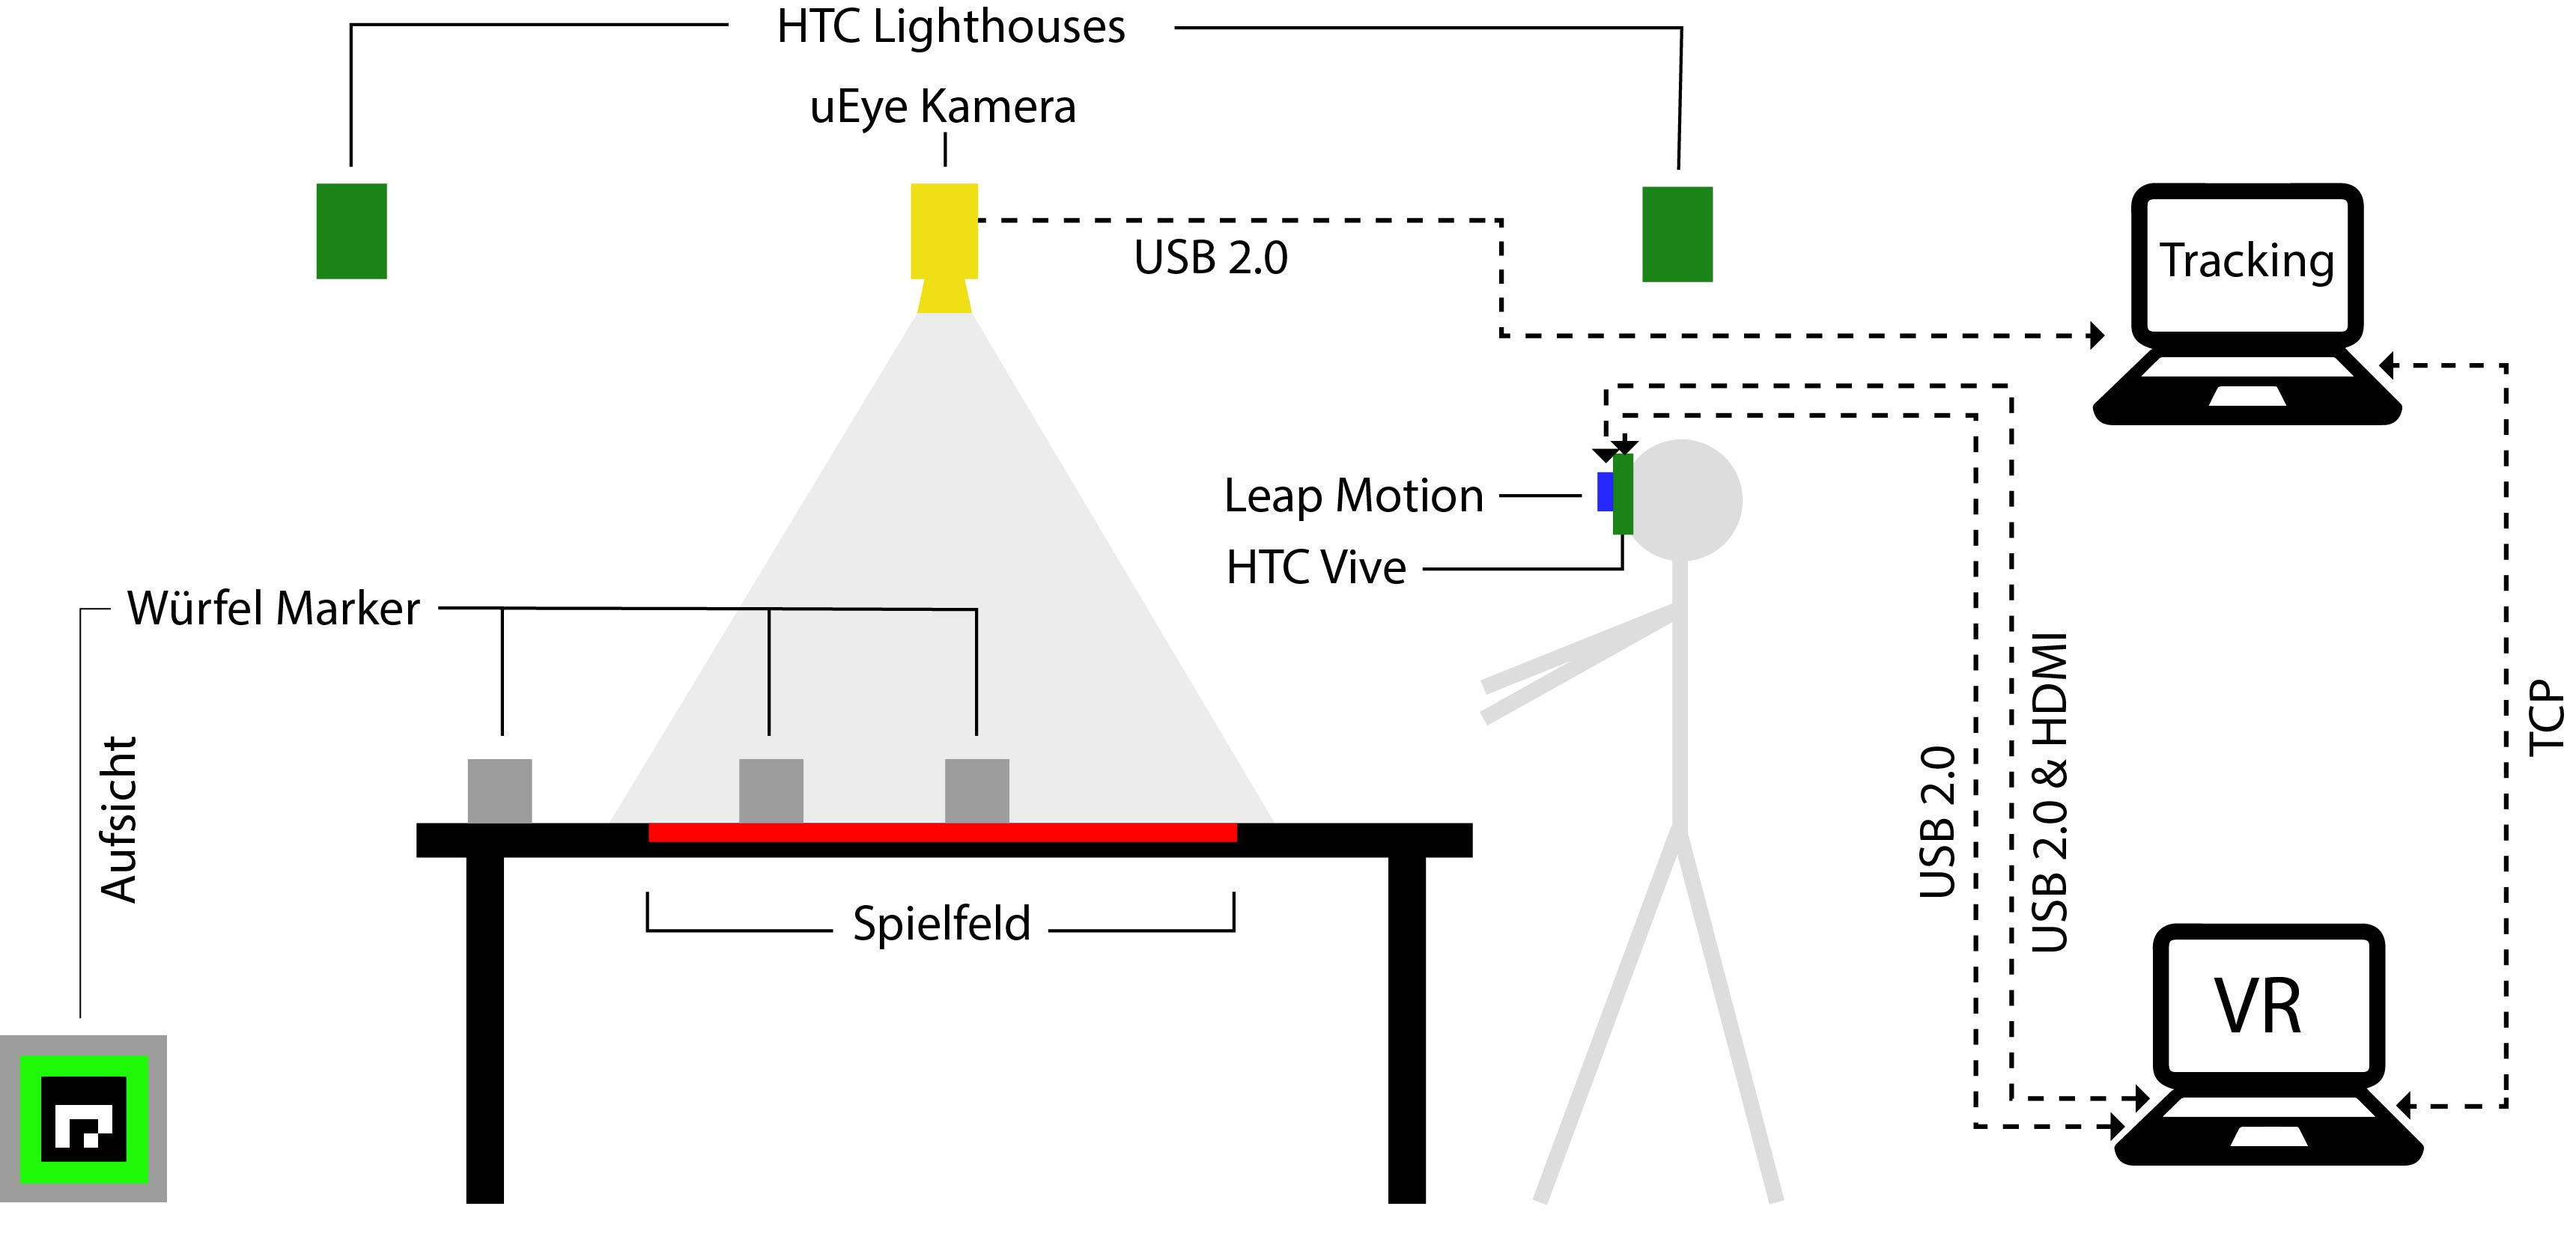
\includegraphics[width=\textwidth]{Bilder/Aufbau_MArC.jpg}
	\caption{Aufbau des \textit{MArC} System.}
	\label{fig:AufbauMarc}
\end{figure}

\begin{figure}[H]
	\centering
	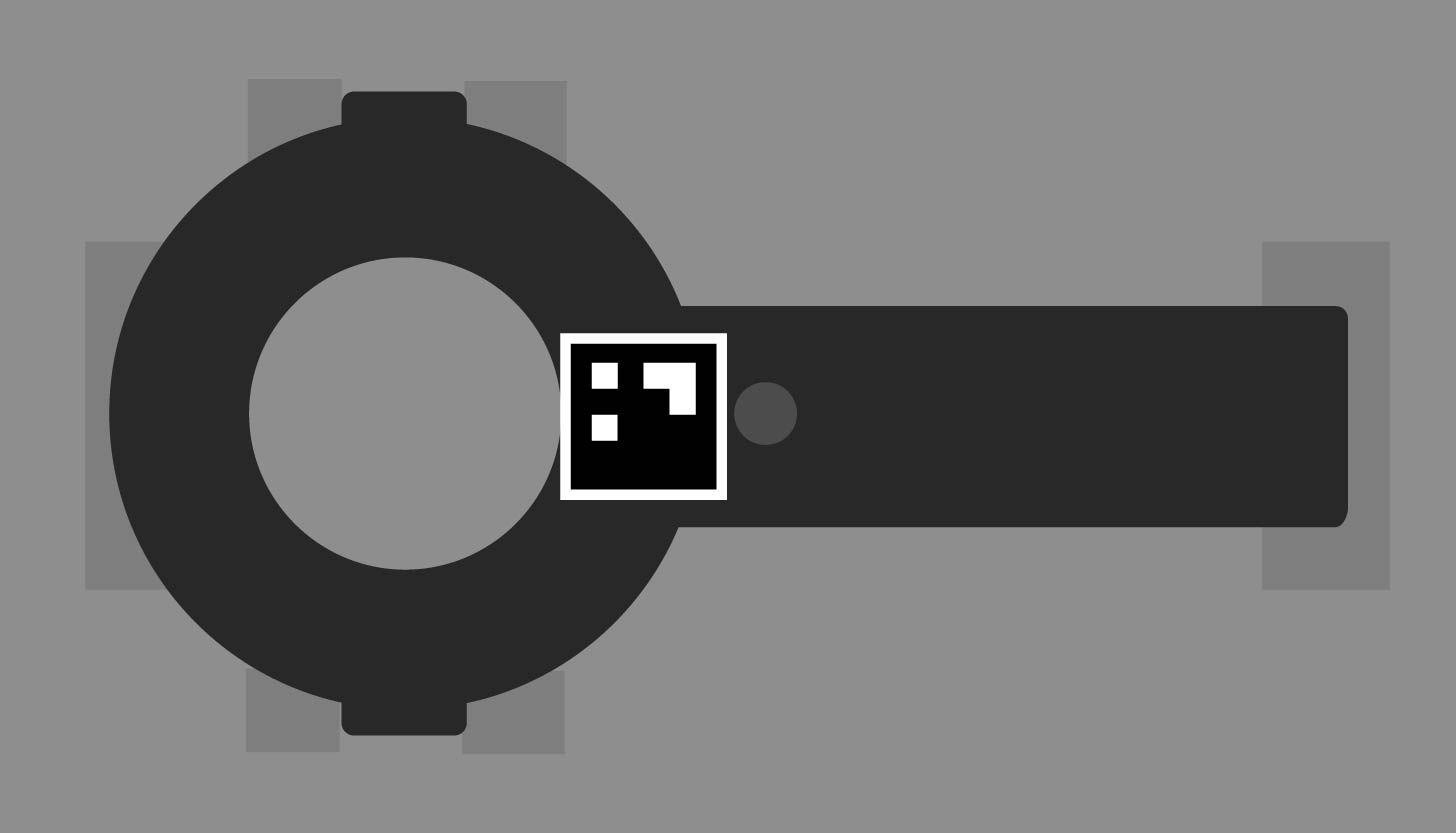
\includegraphics[width=4in]{Bilder/CalibController.jpg}
	\caption{Kalibrierungscontroller des \textit{MArC} System mit ArUco Marker.}
	\label{fig:KontrollerMarc}
\end{figure}

\subsection{Systemvoraussetzungen}\label{sec:sysVor}\todo[inline, color=green]{Lukas}
Die Systemvoraussetzungen für \emph{MArC} sind in der ReadMe-Datei beschrieben, welche der im Projekt erstellten Software mitgeliefert ist. Die gesamte ReadMe-Datei ist in Abschnitt~\ref{sec:readMe} zu finden, außerdem enthält Abbildung~\ref{fig:marcReadMe} einen Ausschnitt der ReadMe-Datei, welcher die Voraussetzungen beschreibt, die vor dem Starten des Systems erfüllt sein müssen.

\begin{figure}
	\centering
	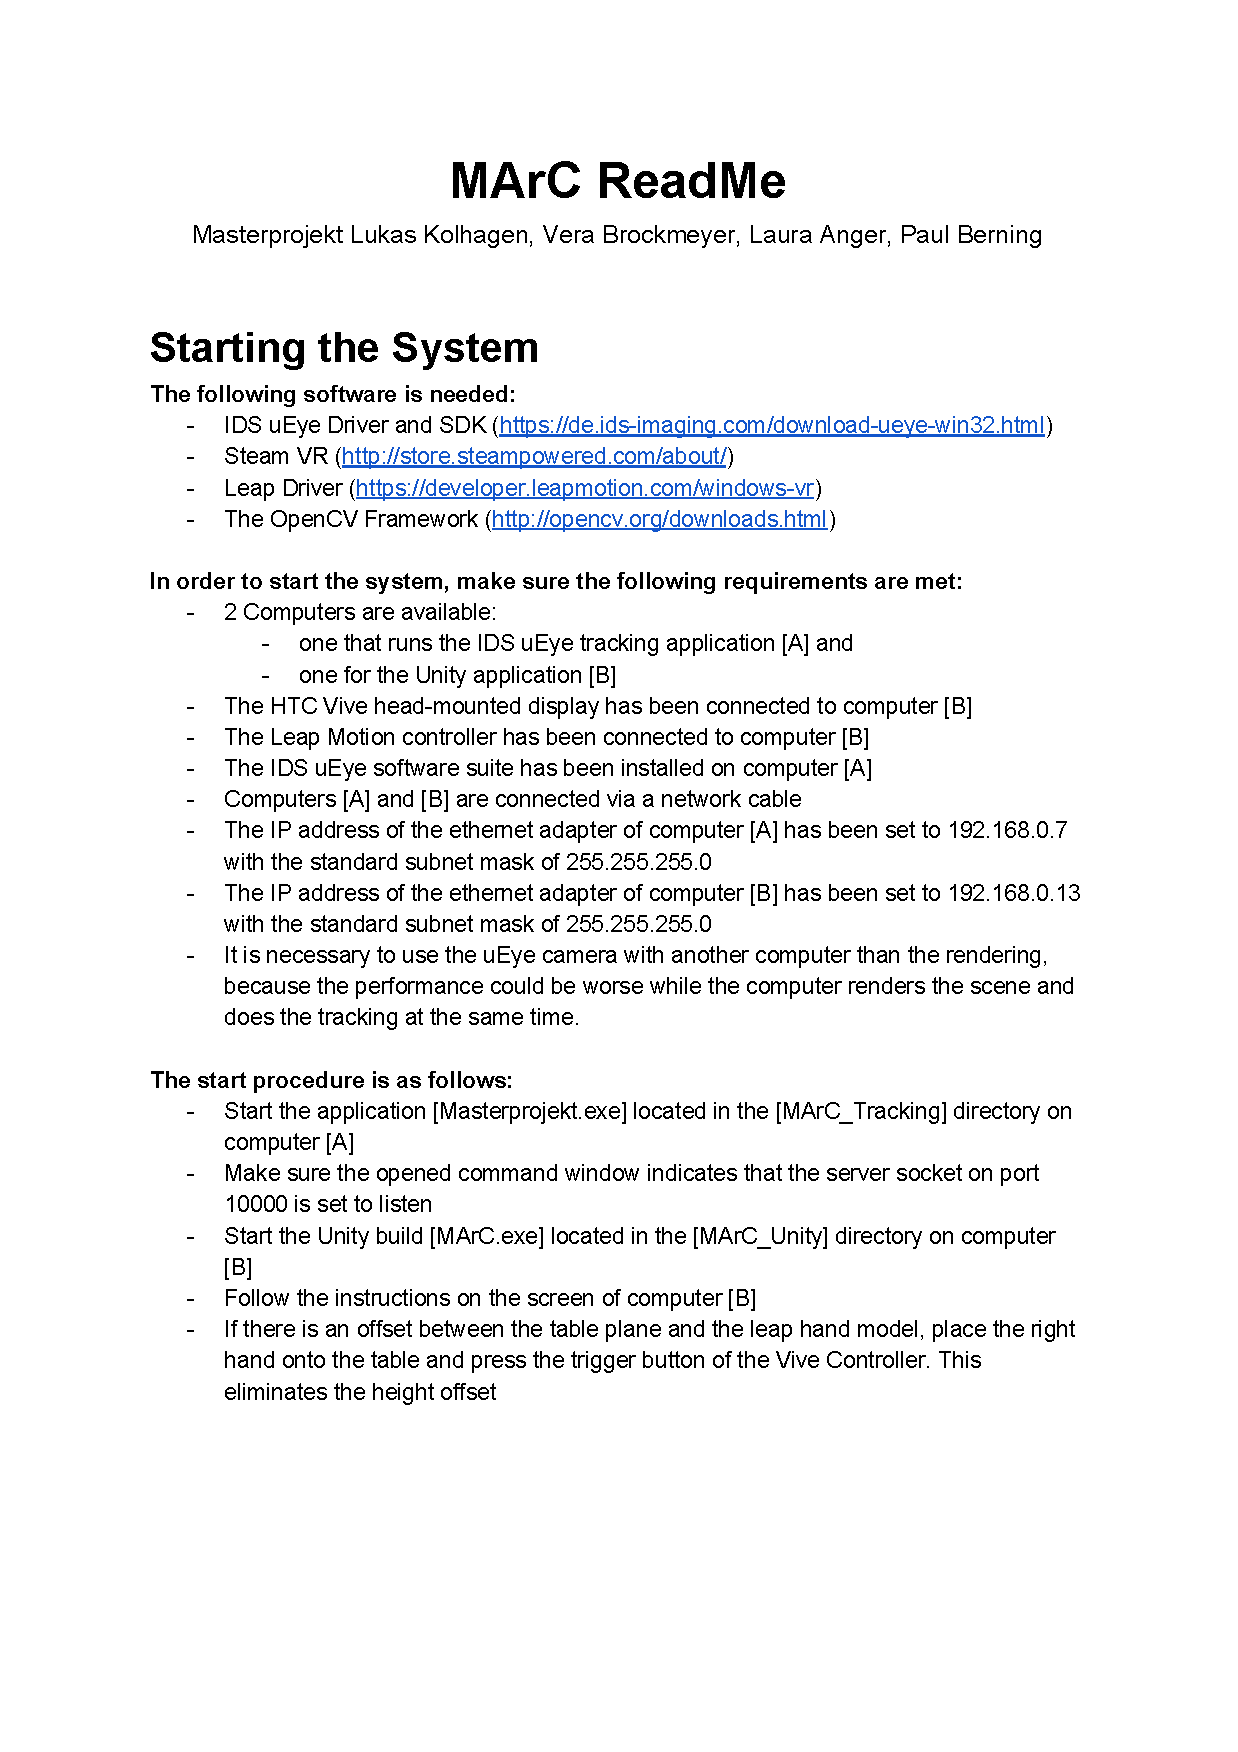
\includegraphics[page=1, trim=1cm 12.25cm 1cm 5.25cm, clip, width=\textwidth]{kapitel/anhang/ReadMe.pdf} 
	\caption{Auszug aus der \emph{MArC} ReadMe-Datei (vgl.~\ref{sec:readMe}).}
	\label{fig:marcReadMe}
\end{figure}

\subsection{Netzwerk}\label{sec:netzwerk}\todo[inline, color=green]{Lukas und Laura}

Die in Kapitel \ref{sec:Winsock} beschriebene API stellt die Möglichkeit bereit, den Datentransport mittels TCP oder UDP zu verwenden. Für \emph{MArC} wurde ein TCP-Socket-Netzwerk bestehend aus (genau) einem Server und (genau) einem Client verwendet, weil der der in~\ref{sec:Netzwerk} beschriebene Fehlerschutz des TCP ausgenutzt werden sollte, um nicht manuell überprüfen zu müssen, ob Daten fehlerfrei übertragen wurden. Da die zu übertragende Datenmenge von \emph{MArC} hinreichend klein -- und von konstanter Größe -- ist, wurde die etwas höhere Geschwindigkeit durch den geringeren Overhead einer UDP-Socket-Verbindung als unnötig erachtet.\\
In den beiden folgenden Abschnitten wird die Umsetzung der Netzwerk-Endpunkte an den beiden für \emph{MArC} verwendeten Computern beschrieben.
\subsubsection{Serverseitige Netzwerkanbindung}\todo[inline]{Laura}
\subsubsection{Client-seitige Netzwerkanbindung}\todo[inline, color=green]{Lukas}
\paragraph{Aufbauen der Netzwerkverbindung}
Das Aufbauen der Netzwerkverbindung vom Client zum Server, also von der Unity-Anwendung zur Tracking-Anwendung, geschieht mit Hilfe der von Winsock (vgl. Abschnitt~\ref{sec:Winsock}) bereitgestellten Klasse \texttt{System.Net.Sockets.TcpClient} wie in Quellcode-Auszug~\ref{lst:setupSocket} dargestellt. Die Netzwerkverbindung wird zu einer fest vorgegebenen IP-Adresse hergestellt.

\lstinputlisting[title=\lstname, caption={\texttt{setupSocket()}-Methode in \texttt{readInNetWorkData.cs}}, label=lst:setupSocket, language={[Sharp]C}, linerange=69-79, firstnumber=69]{Quellcode/readInNetworkData.cs}

\paragraph{Datenübertragung}
Nach einer erfolgreich hergestellten Verbindung sieht das Netzwerkmodul in \emph{MArC} sowohl eine Übertragung von verschiedenen Status, als auch die Übertragung der Tracking-Daten für die Simulation.

\lstinputlisting[title=\lstname, caption={\texttt{sendTCPstatus()}-Methode in \texttt{readInNetWorkData.cs}}, label=lst:sendStatus, language={[Sharp]C}, linerange=81-89, firstnumber=81]{Quellcode/readInNetworkData.cs}

Das Senden und Empfangen von Status seitens der Unity-Anwendung ist in den Quellcode-Auszügen~\ref{lst:sendStatus} und~\ref{lst:receiveStatus} dargelegt. Die Methode zum Senden eines Status ist selbsterklärend. Die \texttt{receiveTCPstatus()}-Methode prüft zunächst, ob eine Netzwerkverbindung hergestellt, also das Socket bereit ist. Anschließend werden genau vier Bytes vom Netzwerk-Datenstrom gelesen, als 32-Bit-Integer interpretiert und zurückgegeben.

\lstinputlisting[title=\lstname, caption={\texttt{receiveTCPstatus()}-Methode in \texttt{readInNetWorkData.cs}}, label=lst:receiveStatus, language={[Sharp]C}, linerange=91-106, firstnumber=91]{Quellcode/readInNetworkData.cs}

Das Empfangen und Interpretieren der Tracking-Daten, nachdem die Simulation gestartet wurde, gestaltet sich ein wenig komplexer und ist im Quellcode-Auszug~\ref{lst:interpretData} aufgeführt. Der Auszug wurde aus Platzgründen in den Anhang verschoben.\\
In der Methode \texttt{interpretTCPMarkerData()} wird ein Byte-Puffer konstanter Länge, welcher vorher vom Netzwerk-Datenstrom gelesen wurde, dahingehend interpretiert, dass anschließend die Daten für alle aktiven Tracking-Marker in geeigneter Form zur weiteren Verarbeitung vorliegen. Als geeignete Form ist hier die Klasse \texttt{Marker} zu nennen, welche als Attribute die ID, die X- und Y-Position, den Winkel und den Status des jeweiligen Markers enthält.\\ 
Beim Interpretieren der Marker werden zunächst die ersten vier Bytes an der von der Schleife abhängigen Pufferposition als ID interpretiert. Sofern die ID gleich $-1$ ist, wird der aktuelle Schleifendurchlauf beendet, da dieser Marker nicht aktiv (valide) ist. Sollte die ID gleich $-2$ sein, indiziert dies, dass für das aktuelle Frame alle Marker übertragen wurden und die Schleife abgebrochen werden kann. In allen anderen Fällen ist die ID valide und alle zusätzlichen Eigenschaften des Markers werden aus dem Puffer gelesen und über den BitConverter geeignet interpretiert. Zuletzt wird ein global angelegtes \texttt{Marker}-Array in jedem Schleifendurchlauf mit dem verarbeiteten Marker befüllt. Bei anschließendem Rendern der Simulation wird dann nur noch auf die so aufbereiteten Daten~--~und nicht mehr auf die Netzwerkdaten~--~zugegriffen.

\subsection{Starten des Systems}\todo[inline, color=green]{Lukas}
Nachdem sichergestellt wurde, dass alle in~\ref{sec:sysVor} beschriebenen Voraussetzungen bestehen, kann das System gestartet werden, indem zunächst die Tracking-Anwendung (auf dem einen Computer, vgl.~\ref{sec:TrackingComp}) und anschließend die aus Unity heraus erstellte Anwendung (auf dem anderen Computer, vgl.~\ref{sec:UnityComp}) gestartet wird. Auf letzterem Computer beginnt darauffolgend die Menüführung, welche in \ref{sec:menu} beschrieben ist. 
\subsection{Menüführung}\label{sec:menu}\todo[inline, color=green]{Lukas}
Die Menüführung dient dazu, den Benutzer durch alle notwendigen Schritte zu leiten, die vor dem Starten der eigentlichen Simulation erforderlich sind. Im nachfolgenden Abschnitt~\ref{sec:menus} werden alle verfügbaren Menüs der Anwendung aufgelistet und kurz beschrieben, während im Abschnitt~\ref{sec:menuAblauf} der Ablauf der Menüführung erläutert wird.


\subsubsection{Menüs}\label{sec:menus}\todo[inline, backgroundcolor=green]{Laura}
Die folgenden Menüs sind Bestandteil der Menüführung:

\begin{minipage}{0.6\textwidth}
	\begin{figure}[H] 
		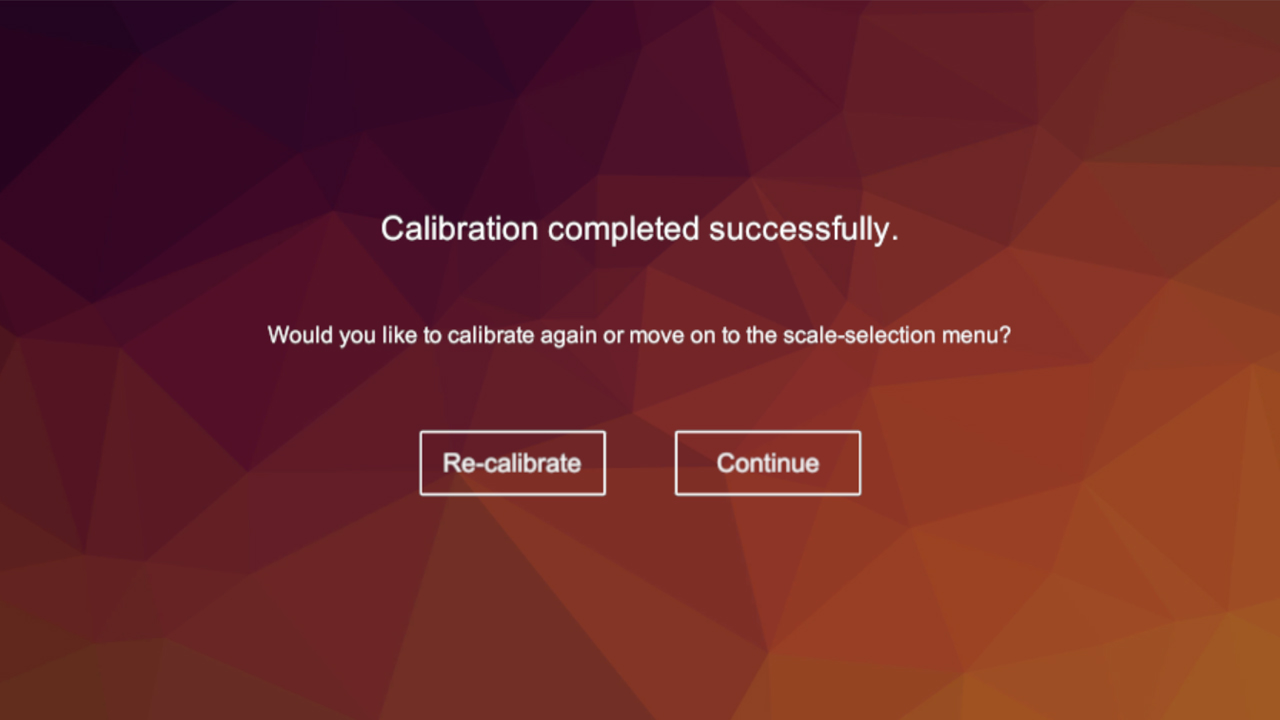
\includegraphics[trim=3cm 2cm 3cm 2cm, clip, width=0.9\textwidth]{Bilder/CalibDone.jpg}
			\label{fig:CalibDone}
	\end{figure}
\end{minipage}
\begin{minipage}{0.4\textwidth}
	\texttt{CalibDone}:\\
	Wird aufgerufen, wenn die Kalibrierung des Arbeitsbereichs abgeschlossen ist. Es informiert den Benutzer, dass die Kalibrierung erfolgreich war und der Vorgang fortgesetzt werden kann.
\end{minipage}\\

\begin{minipage}{0.6\textwidth}
	\begin{figure}[H] 
		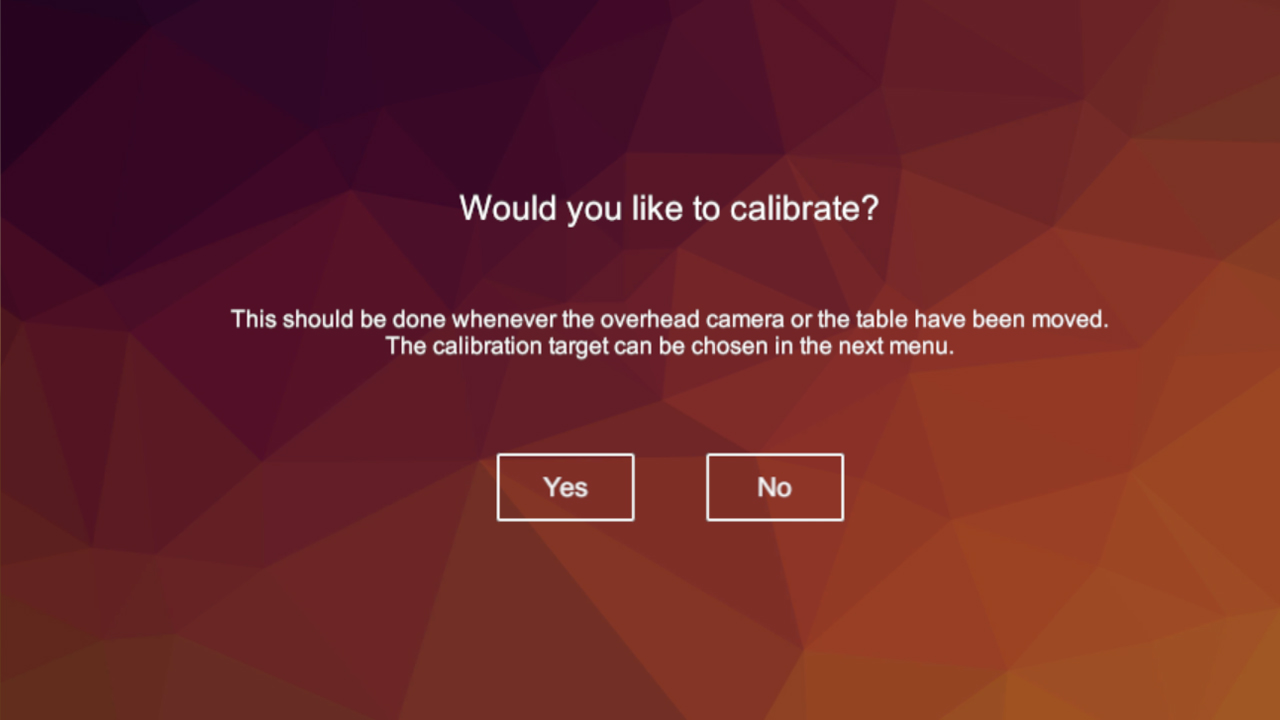
\includegraphics[trim=3cm 2cm 2cm 2cm, clip, width=0.9\textwidth]{Bilder/CalibrateOrNot.jpg}
			\label{fig:CalibrateOrNot}
	\end{figure}
\end{minipage}
\begin{minipage}{0.4\textwidth}
	\texttt{CalibrateOrNot}:\\
	Erscheint nach dem Verlassen des \texttt{Welcome}-Menüs und erlaubt dem Benutzer eine Kalibrierung durchzuführen oder eine bereits durchgeführte Kalibrierung zu laden.
\end{minipage}\\

\begin{minipage}{0.6\textwidth}
	\begin{figure}[H] 
		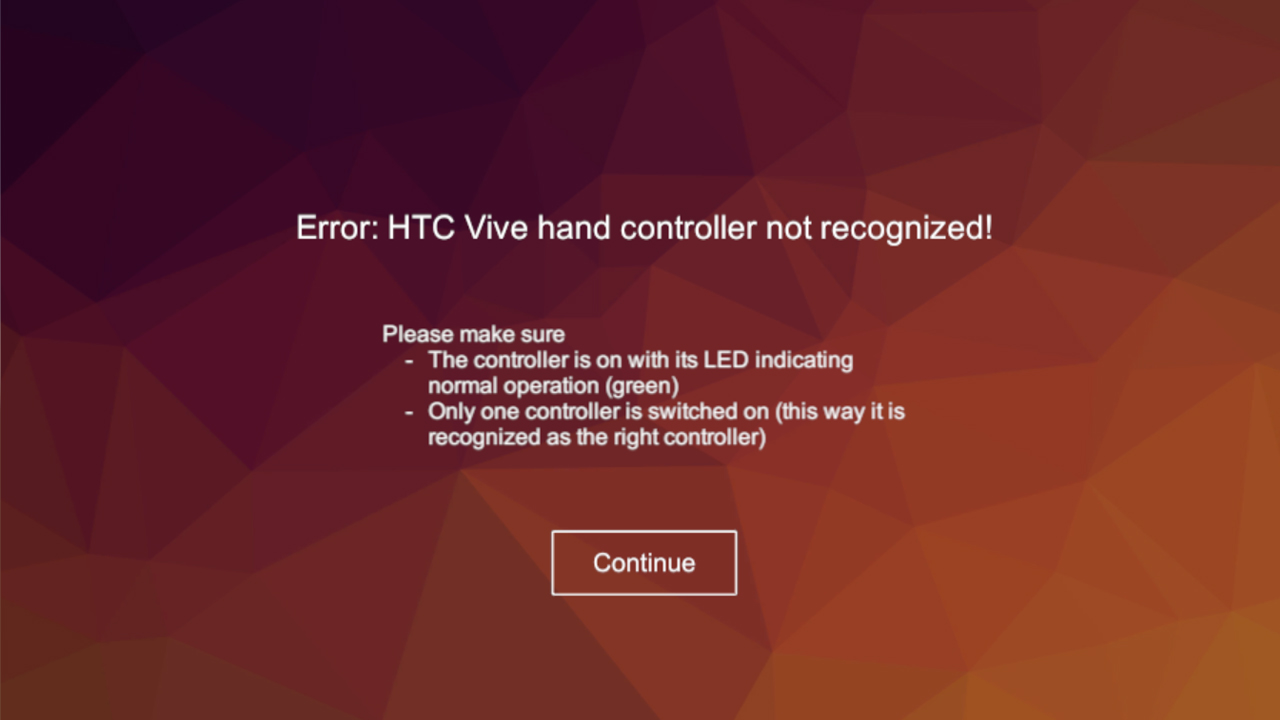
\includegraphics[trim=3cm 1cm 3cm 3cm, clip, width=0.9\textwidth]{Bilder/ControllerNotFound.jpg}
			\label{fig:ControllerNotFound}
	\end{figure}
\end{minipage}
\begin{minipage}{0.4\textwidth}
	\texttt{ControllerNotFound}:\\
	Warnt den Benutzer nach dem Starten der Kalibrierung, dass der HTC Vive Controller, welcher für die Kalibrierung benötigt wird, nicht eingeschaltet ist. Während das Menü angezeigt wird, kann der Benutzer den Controller einschalten und anschließend auf \texttt{Continue} klicken.
\end{minipage}\\

\begin{minipage}{0.6\textwidth}
	\begin{figure}[H] 
		\includegraphics[trim=3cm 1cm 3cm 3cm, clip, width=0.9\textwidth]{Bilder/doPlaneCalibInVS.jpg}
			\label{fig:doPlaneCalibInVS}
	\end{figure}
\end{minipage}
\begin{minipage}{0.4\textwidth}
	\texttt{doPlaneCalibInVS}:\\
	Dient dem Benutzer als Anleitung für die Durchführung der Arbeitsbereich-Kalibrierung. Diese wird in \ref{sec:planeCalib} genauer beschrieben.
\end{minipage}\\

\begin{minipage}{0.6\textwidth}
	\begin{figure}[H] 
		\includegraphics[trim=3cm 2cm 3cm 2cm, clip, width=0.9\textwidth]{Bilder/doPoseCalibInVS.jpg}
			\label{fig:doPoseCalibInVS}
	\end{figure}
\end{minipage}
\begin{minipage}{0.4\textwidth}
	\texttt{doPoseCalibInVS}:\\
	Dient dem Benutzer als Anleitung für die Durchführung der Kamera-Kalibrierung. Diese wird in \ref{sec:camCalib} genauer beschrieben.
\end{minipage}\\

\begin{minipage}{0.6\textwidth}
	\begin{figure}[H] 
		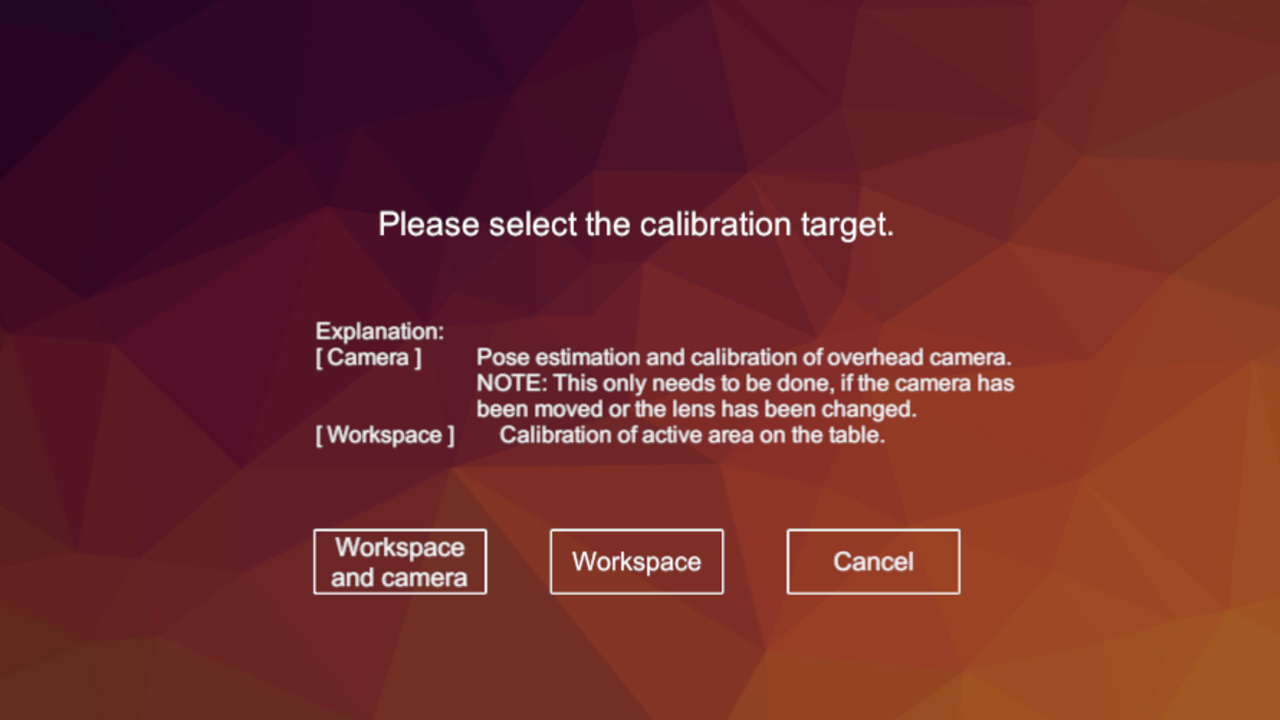
\includegraphics[trim=3cm 1cm 3cm 3cm, clip, width=0.9\textwidth]{Bilder/SelectCalibrationTarget.jpg}
			\label{fig:SelectCalibrationTarget}
	\end{figure}
\end{minipage}
\begin{minipage}{0.4\textwidth}
	\texttt{SelectCalibrationTarget}:\\
	Erlaubt die Auswahl der Art der Kalibrierung. Es kann hier entweder nur der Arbeitsbereich oder sowohl der Arbeitsbereich, als auch die Kamera kalibriert werden. Die Kalibrierung ist näher in \ref{sec:calib} beschrieben.
\end{minipage}\\

\begin{minipage}{0.6\textwidth}
	\begin{figure}[H] 
		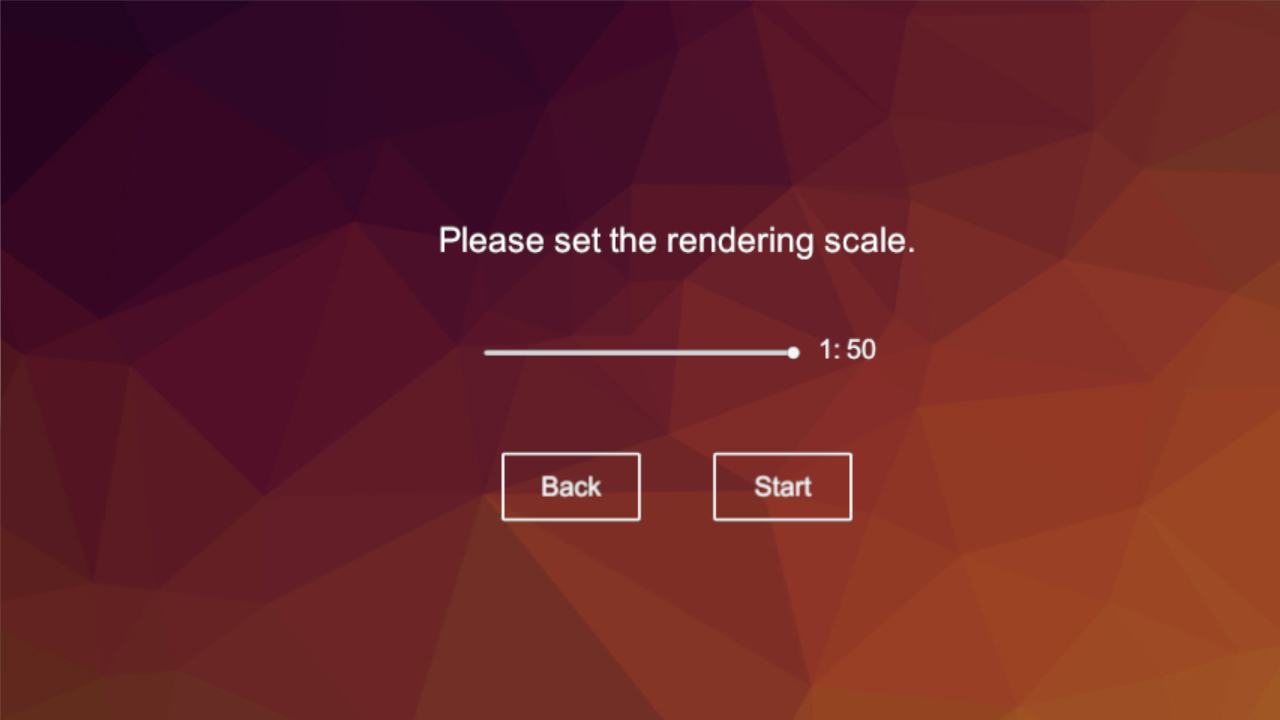
\includegraphics[trim=3.5cm 1cm 2.5cm 3cm, clip, width=0.9\textwidth]{Bilder/SetScale.jpg}
			\label{fig:SetScale}
	\end{figure}
\end{minipage}
\begin{minipage}{0.4\textwidth}
	\texttt{SetScale}:\\
	Stellt das letzte Menü vor dem Starten der Simulation dar. In diesem kann der Benutzer den Maßstab der Gebäudesimulation einstellen und anschließend die Simulation starten.
\end{minipage}\\

\begin{minipage}{0.6\textwidth}
	\begin{figure}[H] 
		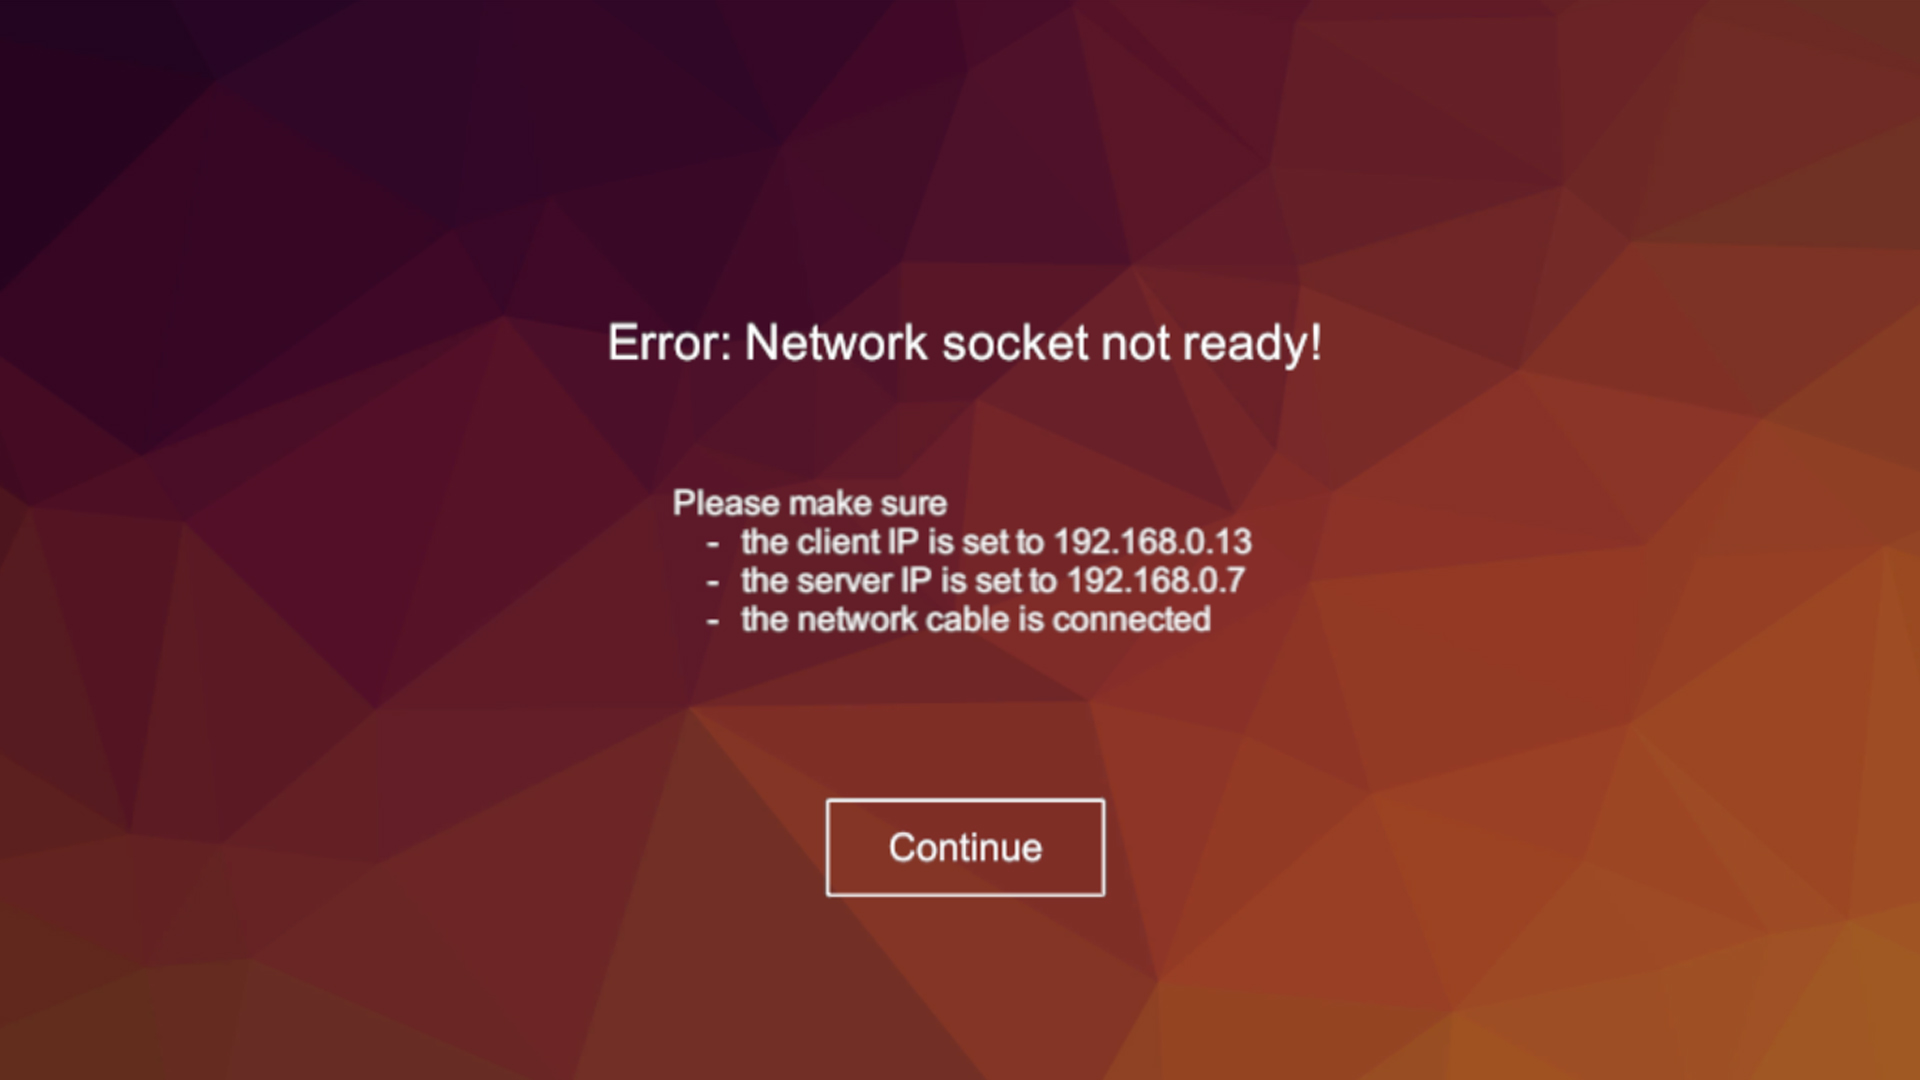
\includegraphics[trim=3cm 1cm 3cm 3cm, clip, width=0.9\textwidth]{Bilder/SocketNotReady.jpg}
			\label{fig:SocketNotReady}
	\end{figure}
\end{minipage}
\begin{minipage}{0.4\textwidth}
	\texttt{SocketNotReady}:\\
	Warnt den Benutzer nach dem Verlassen des \texttt{Welcome}-Menüs, dass die Netzwerkverbindung zwischen den beiden Computern nicht bereit ist. Nach Bestätigung dieses Hinweises durch einen Klick auf \texttt{Continue}, kehrt der Benutzer zum \texttt{Welcome}-Menü zurück. %Anschließend kann der Vorgang fortgesetzt werden, wenn die Netzwerkverbindung hergestellt wurde. Andernfalls erscheint wieder \texttt{SocketNotReady}.
\end{minipage}\\

\begin{minipage}{0.6\textwidth}
	\begin{figure}[H] 
		
\includegraphics[trim=3cm 2cm 3cm 2cm, clip, width=0.9\textwidth]{Bilder/Welcome.jpg}
			\label{fig:Welcome}
	\end{figure}
\end{minipage}
\begin{minipage}{0.4\textwidth}
	\texttt{Welcome}:\\
	Erscheint als erstes Menü. Hier erhält der Nutzer eine kurze Information darüber, wie die Anwendung heißt und wozu sie dient.
\end{minipage}\\

\subsubsection{Ablauf der Menüführung}\label{sec:menuAblauf}\todo[inline, color=green]{Lukas}
Der Ablauf der Menüführung von \textit{MArC} ist in Abbildung~\ref{fig:menuFlow} dargestellt. Die einzelnen Menüs sind bereits in~\ref{sec:menus} beschrieben worden.

\begin{figure}[htbp]
	\centering
	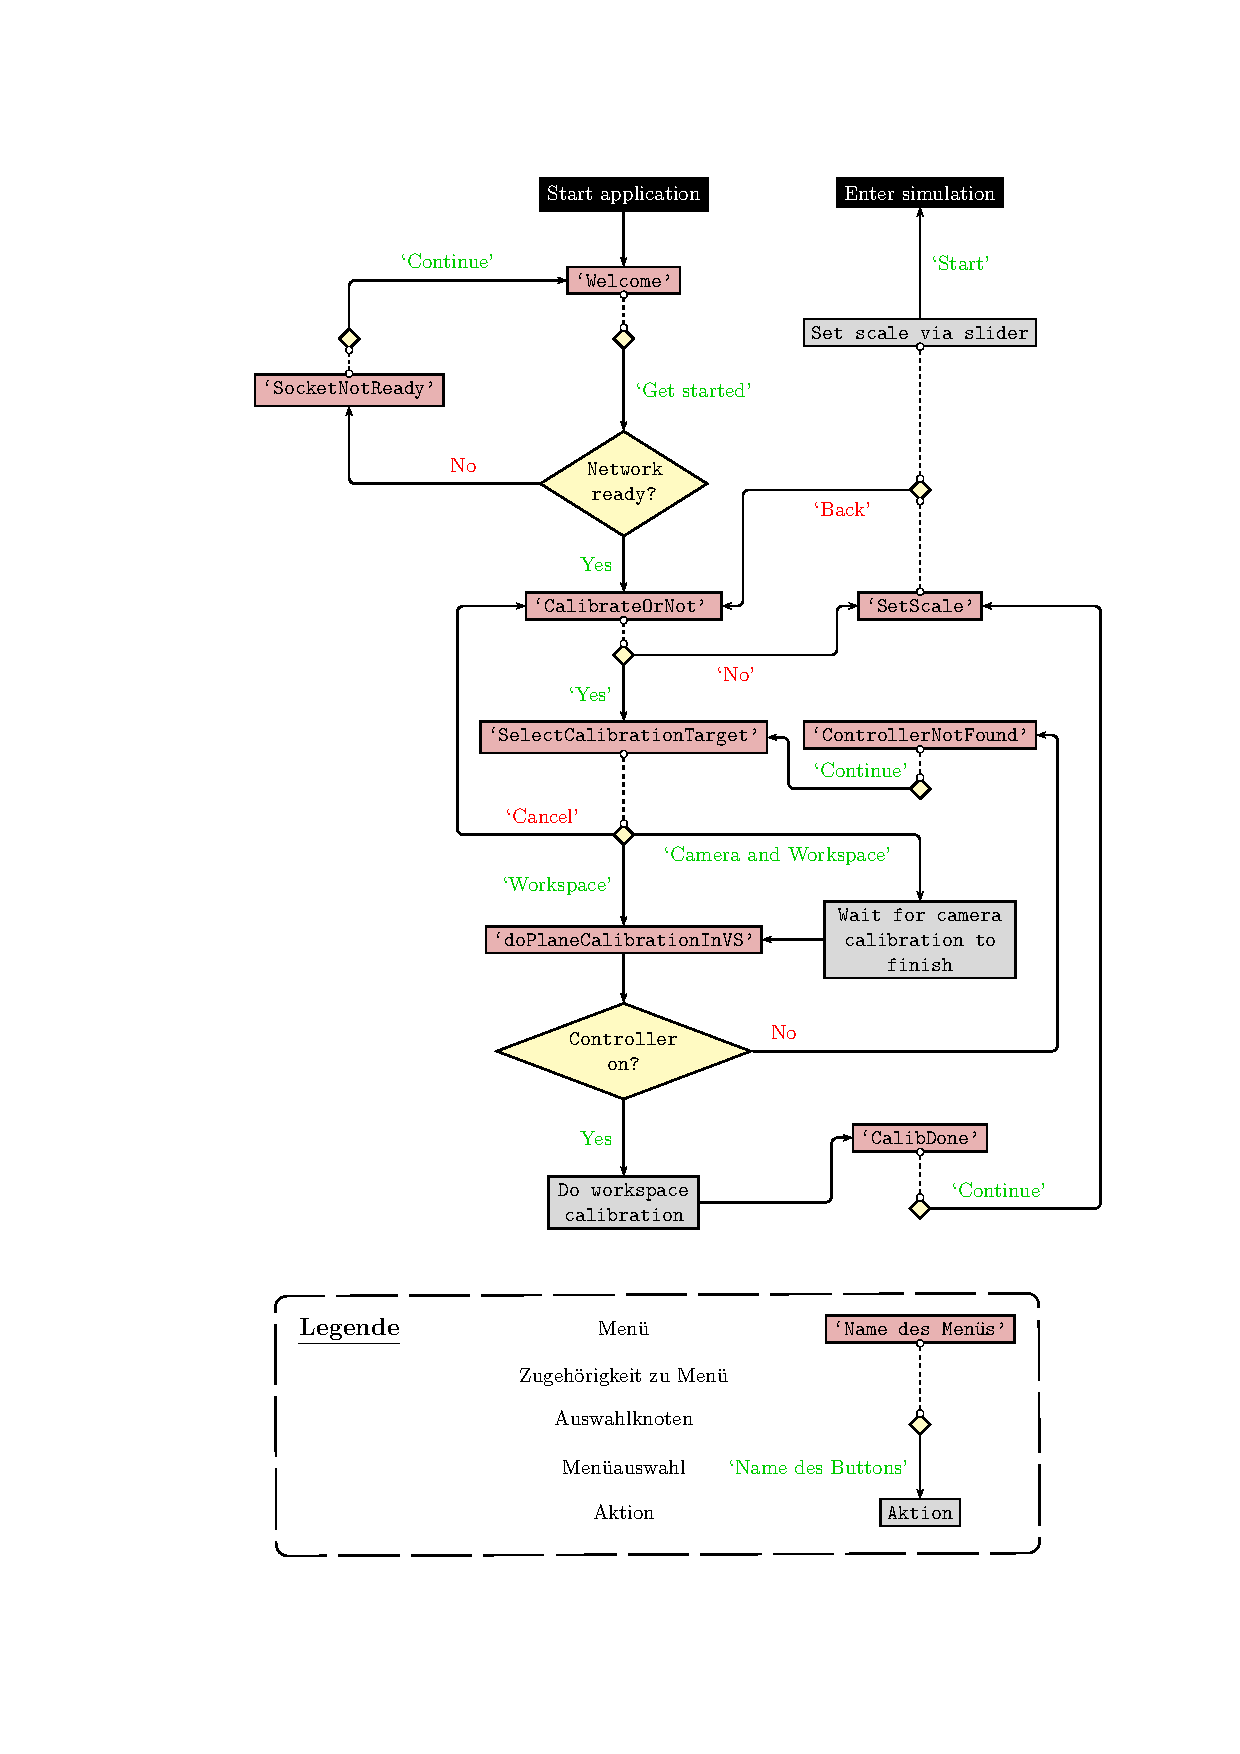
\includegraphics[scale=.9, trim=5.5cm 2.5cm 3.5cm 2.5cm]{kapitel/system/MP_Menu_Flowchart.pdf}
	\caption{Flussdiagramm der Menüführung.}
	\label{fig:menuFlow}
\end{figure}

Nach dem Starten der Anwendung wird zunächst das Menü \texttt{Welcome} angezeigt. Dieses enthält nur einen Button \textit{Get started}. Sobald dieser gedrückt wird, prüft die Anwendung, ob eine Netzwerkverbindung zu dem Computer mit der Tracking-Anwendung besteht. Sollte dies nicht der Fall sein, wird das Menü \texttt{Socket\-Not\-Ready} angezeigt. Dieses verlässt der Benutzer über einen Klick auf \texttt{Continue}, anschließend wird erneut das Menu \texttt{Welcome} angezeigt. Wenn zu diesem Zeitpunkt die Netzwerkverbindung korrekt hergestellt wurde, gelangt der Benutzer zum Menü \texttt{Calibrate\-Or\-Not}, anderenfalls wird wiederholt \texttt{Socket\-Not\-Ready} angezeigt.

In \texttt{CalibrateOrNot} hat der Benutzer die Auswahl zwischen den Schaltflächen \textit{Yes} und \textit{No}. Bei einem Klick auf \textit{Yes} wird anschließend \texttt{Select\-Calibration\-Target} angezeigt, bei einem Klick auf \textit{No} lädt das System eine zuvor durchgeführte Kalibrierung und das Menü \texttt{Set\-Scale} wird geöffnet.

\texttt{Select\-Calibration\-Target} stellt den Benutzer vor die Wahl entweder nur den Arbeitsbereich (\textit{Work\-space}) oder sowohl den Arbeitsbereich als auch die Kamera zu kalibrieren (\textit{Camera and Workspace}). Außerdem besteht die Möglichkeit über \textit{Cancel} zum Menü \texttt{Calibrate\-Or\-Not} zurückzukehren.

Wählt der Benutzer \textit{Camera and Workspace} in \texttt{Select\-Calibration\-Target} aus, so informiert die Anwendung die Tracking-Anwendung auf dem anderen Computer und wartet anschließend darauf, dass von dort die Bestätigung gesendet wird, dass die Kamerakalibrierung abgeschlossen ist. Anschließend wird das Menü \texttt{doPlane\-Calibration\-InVS} angezeigt, welches auch aufgerufen wird, wenn der Benutzer \textit{Work\-space} in \texttt{Select\-Calibration\-Target} wählt.

Im Menü \texttt{doPlane\-Calibration\-InVS} wird zunächst geprüft, ob der für die Kalibrierung notwendige HTC Vive Controller eingeschaltet ist. Sollte dies nicht der Fall sein, wird \texttt{Controller\-Not\-Found} aufgerufen. Dieses kann mit einem Klick auf \textit{Continue} verlassen werden, woraufhin wieder \texttt{Select\-Calibration\-Target} angezeigt wird.\\
Sofern der HTC Vive Controller beim Aufruf von \texttt{doPlane\-Calibration\-InVS} eingeschaltet ist, wird nach Durchführung der Kalibrierung des Arbeitsbereichs das Menü \texttt{CalibDone} angezeigt.

\texttt{Calib\-Done} kann über einen Klick auf \textit{Continue} verlassen werden und führt den Nutzer anschließend zu \texttt{SetScale}. Aus diesem Menü kann über den Button \textit{Back} entweder zu \texttt{CalibrateOrNot} zurückgekehrt oder die Simulation mit dem im Menü über den Slider eingestellten Maßstab gestartet werden.



\subsection{Kontextmenü}\label{sec:kontextMenu}\todo[inline]{Laura und Lukas}

\subsection{Marker Handles}\label{sec:markerHandles}\todo[inline]{Paul}
Jeder Marker verfügt über die Möglichkeit in seiner Größe in X-, Y- und Z-Achse verändert zu werden. Diese sog. "Handles" sind sichtbar, wenn das Kontextmenü angezeigt wird (s. Abschnitt  \ref{KontextMenü}. Die Handles bestehen aus Zylindern, die mit einem Collider versehen wurden. Die X- und Y- Achse wird betätigt, indem der Benutzer mit einem Finger das jeweiligen Handle berührt und dann in die entsprechende Richtung zieht. Die Größe in Z-Achse wird über "+" und "-" Button gesteuert. Drückt der Benutzer diese Buttons, wird das Gebäude um je ein Stockwerk erhöht oder verniedrigt. \\
Die Interaktion der Handles mit der Hand des Nutzers wurde über das Leap-Handmodell umgesetzt; dieses besitzt Collider, die an den Fingern des Modells angebracht sind und sich simultan mit der Hand des Nutzers bewegen. Berührt die Hand nun einen der Handler, wird dieser Collider des Handlers "angesprochen". Im Falle der X-, und Y-Handles wird in der \texttt{update} Funktion des Skripts \texttt{contextMenuTrigger.cs} ein Vektor berechnet, der die Start und Endposition der Bewegung miteinander verrechnet. Im Falle einer Bewegung in X Position wird die sog. "localDifference" berechnet, dies ist der Abstand des Fingers zur Position des Markers. Die eigentliche Skalierung wird dann wie folgt berechnet:\\
\begin{equation}
pos = (startPosition.x - localDifference.y) / 2, startPosition.y, startPosition.z)
\end{equation}

Das Gebäude wird dann um den Vektor pos im lokalen Objektkoordinatensystem vergrößert.\\
Für die Bewegung in Y berechnet sich der Vektor wie folgt:

\begin{equation}
pos = (startPosition.x , startPosition.y, (startPosition.z - localDifference.y) / 2)
\end{equation}

Es fällt auf, dass in der zu verändernden Achse verschiedene Achsen zur Berechnung verwendet werden müssen. Dies kommt daher, dass das Koordinatensystem der Leap Motion nicht equivalent zu dem in Unity ist.\\
Dass der Wert der zu verändernden Achse halbiert wird, hat sich empirisch als Sinnvoll herausgestellt. Ohne diese "Übersetzung" der Bewegung würde das Gebäude nicht equivalent zur Fingerbewegung vergrößert oder verkleinert werden. 

\subsubsection{Menüführung}\todo[inline]{Laura}
\subsubsection{Architektur Berechnung}\todo[inline]{Laura}


\subsection{Table Menü}\label{sec:TableMenü}\todo[inline, color=yellow]{Paul}

Zur intuitiven Bedienung des \textit{MArC} wurden die Menüs, die während der Laufzeit benutzt werden können, auf dem Arbeitstisch platziert. Dies hat den Vorteil, dass zum einen diese Menüs permanent sichtbar sein können, ohne den Nutzer während der Arbeit zu stören und zum anderen ein haptisches Feedback bei der Nutzung möglich ist.\\
Möchte der Nutzer die Menüs bedienen, so drückt er mit dem Finger, der durch die \textit{Leap Motion} getrackt wird auf die Buttons und damit gleichzeitig auf den Tisch. Dies erleichtert die Benutzung deutlich im Vergleich zu der Nutzung von Menüs die im Raum schweben.\\
Im laufe der Entwicklung hat sich für das rechte Menü der Name \textit{Table Menü} etabliert. Im folgenden wird dessen Funktion im Detail erläutert.

\subsubsection{Szenen Management}\todo[inline, color=green]{Paul}
Eine Anforderung an das System war, dass der Nutzer erstellte Szenen abspeichern und wieder aufrufen können soll. Anhand des \textit{Table Menüs} ist dies möglich. Die Funktionen des Menüs sind:
\begin{itemize}
	\item Speichern von Szenen
	\item Laden von Szenen und aufrufen des \textit{Match Modus} (s. Abschnitt \ref{MatchModus})
	\item Scrollen durch die gespeicherten Szenen

\end{itemize}



\subsubsection{Speichern von Szenen}\todo[inline, color=green]{Paul}
\label{Speichern}
Möchte der Nutzer eine Szene speichern, so drückt er mit dem Finger auf den Button \glqq Save \grqq{}. \textit{MArC} speichert die aktuelle Szene automatisch in dem Ordner \glqq \textbackslash Resources\textbackslash saves\textbackslash Dateiname.xml\grqq{}.\\
Der Dateiame setzt sich aus aktuellem Datum und aktueller Zeit zum Speicherzeitpunkt wie folgt zusammen:
\begin{center}
	\texttt{Tag-Monat-Jahr-Stunde-Minute-Sekunde.xml}
\end{center}
Durch diese Markierung können später Dateien identifiziert werden, die auch nur Sekunden hintereinander gespeichert wurde.\\
Da innerhalb von \textit{Unity} eine hierarchiche Anordnung sämtlicher Elemente in Form eines Szenegraphen angewendet wird, bot sich eine Speicherung der Daten ebenfalls hierarchich in form eines XML Dokumentes an.\\
Die \textit{Extensible markup language (XML)} beschreibt eine Klasse von Daten Objekten (XML Documents) und ermöglicht das hierarchiche Abspeichern von geparsten oder ungeparsten Daten \cite{bray1998extensible}. In \textit{C\#} sind Verarbeitungsklassen bereits implementiert. Mittels dieser sog. \textit{XML Prozessoren} wird ein Datenzugriff erleichtert.

\paragraph{Dateiaufbau einer gespeicherten Szene}
Das gesamte Dokument wird mit einem Hauptknoten  \texttt{ $<$AR2\_COMPOSERSCENE$>$} umspannt. Innerhalb diesem wird mit texttt{ $<$time$>$}
ein Zeitstempel mit gespeichert, falls der Dateiname einmal umbenannt werden sollte.
Anschließend folgt der  texttt{ $<$TableObject$>$} Knoten, innerhalb dessen die Marker gespeichert werden. Jeder Marker wird nach dem folgenden Schema gespeichert, welches den Aufbau in Unity repräsentiert:


 \begin{lstlisting}
	<Name>
		<Kindknoten>
		<PositionX>
		<PositionY>
		<PositionZ>
		<RotationX>
		<RotationY>
		<RotationZ>
		<ScaleX>
		<ScaleY>
		<ScaleZ>
	</Name>
 \end{lstlisting}

Wobei sich dies als Kurzsschreibweise versteht, innerhalb der Positions/Rotations/Scale Knoten ist der entsprechende Wert eingetragen.

\paragraph{Vorgehen der Speicherung}
Das Skript \texttt{save.cs} ist für die Speicherung der Szenen verantwortlich. Zunächst wird der Zeitstempel geseichert und der Dateiname genertiert. Anschließend wird ein neues XML Dokument erstellt. An dieses wird zunächst der äußerste Knoten angehangen sowie der Zeitstempel. Anschließend wird die rekursive Funktion \texttt{traverseHierarchie} mit dem TableObject der Unity Szene aufgerufen und wird für jeden Kindknoten ausgeführt. \\
Diese Funktion erstellt jeweils die Knoten für den Namen, die Position, Rotation und Skalierung. Die Werte werden mittels \texttt{Node.InnerText} in die Knoten gespeichert.\\
Ist diese Funktion durch alle Kindknoten gegangen, wird am Ende noch die Skalierung der Szene in dem Knoten \texttt{globalBuildingScale} abgespeichert, damit dieser beim Laden der Szene rekonstruiert werden kann.

\paragraph{Darstellen von gespeicherten Szenen} Die gespeicherten Szenen werden in Listenform im Table Menü dargestellt. Zu oberst sind immer die aktuellen Szenen. Über die Buttons "1-6", "7-12", "13-18"  und "19-24" kann "umgeblättert" werden und weitere, in der Vergangenheit liegende Szenen dargestellt werden. Für diese Darstellung ist das Skript \texttt{Timeline.cs} zuständig. Bei jedem Speichern wird die Darstellung aktualisiert, so dass immer alle neuesten gespeicherten Szenen sichtbar sind.

\subsubsection{Laden von Szenen}\todo[inline, color=green]{Paul}
\label{Laden}
Das Laden der Szenen ist ein komplexer Vorgang. Dies kommt daher, dass auf der einen Seite Markerdaten in der zu öffnenden .xml Datei gespeichert sind und geladen werden müssen. Auf der anderen Seite gibt es evt. noch Marker, die auf dem Arbeitsfeld liegen und aktuell getrackt werden. Beide Informationsströme müssen beim laden der Szene berücksichtigt werden und korrekt verarbeitet werden. Ein einfaches übertragen von Positions-, Rotations- und Skalierungsdaten auf vorhandene Markerobjekte ist nicht möglich, da diese permanent durch den TCP Datenstrom überschrieben werden würden.
\paragraph{Vorgehen beim Laden} Durch Auswählen der Datei im Table Menü mit dem Finger wird das Skript \texttt{open.cs} gestartet. Dieses setzt zuerst den Pfad aus dem aktuellem Applikationspfad mit dem Unterordner Resources und saves zusammen und fügt den Namen der zu öffnenden .xml Datei aus dem Table Menü hinzu. Anschließend wird die Datei eingelesen, die internen Knoten liegen dann in einer XmlNodeList bereit. Es wird die Funktion \texttt{crawlXML} aufgerufen.\\
Da aus organisatorischen Gründen alle Marker in der Datei gespeichert werden müssen, wird die XmlNodeList bearbeitet und geprüft, welche der Marker als "aktiv" gespeichert wurden. Aktive Marker sind solche, die zum Zeitpunkt des Speichern sichtbar waren. Alle aktiven Marker werden in der ArrayList activeMarkerIDs gespeichert.\\
Diese ArrayList wird nun, nachdem sie vollständig gefüllt ist, bearbeitet: Für jeden Eintrag, also jeden aktiven Marker wird ein Vorlagemarker instantiiert. Dies ist ein Marker, der bereits alle Komponenten die benötigt werden angeheftet hat und dem nur noch die Parameter zugewiesen werden müssen. Dies wird dann getan; jeder Marker bekommt die OriginalID + 100 als Namen zugewiesen. Dies ist wichtig um später die aus der .xml Datei gelesenen Marker von den aktuell über TCP gesteurten Marker unterscheiden zu können. Anschließend wird werden die weiteren Parameter wie Position, Rotation und Skalierung an den Marker übergeben. Schließlich wird der Marker an das "TableObject" in \textit{Unity} gehangen und sichtbar gemacht. Als letzter Schritt wird die Markervariable "MatchMode" auf "true" gesetzt und das Skript \texttt{matchMode.cs} aktiviert. Dieses wird detailliert im Abschnitt \ref{MatchModus} beschrieben. Die Marker die sich in diesem Match Modus befinden blinken grün und rot, um zu signalisieren, dass sie auf einen "echten" Marker warten.
Sind alle Marker auf diese Weise geladen und parametrisiert, wird der globale Maßstab an das Skript \texttt{setupScene.cs} übergeben.\\
Zu diesem Zeitpunkt sind also zwei Arten von Markern sichtbar: Die geladenen aus der .xml Datei, die grün und rot blinken und eine ID $>$ 100 haben, und die aktiven Marker die getrackt werden.



\subsubsection{Match Modus}\todo[inline,color=green]{Paul}
\label{MatchModus}
Der Match Modus ist ein Systemzustand, der nach dem Laden von gespeicherten Szenen aktiviert wird. Es werden wie im Abschnitt \ref{Laden} beschrieben die geladenen Marker und die getrackten Marker gleichzeitig angezeigt. Der Benutzer muss jetzt die echten Marker an die Position der geladenen virtuellen Marker schieben. Ist ein Marker im Match Modus, sind vier Collider an den Ecken des virtuellen Markers wichtig. Die Markerinterne Variable "matchMode" ist = "false" gesetzt. Schiebt der Benutzer nun einen Marker an die Position des virtuellen Markers, werden bei genauer Positionierung alle vier Collider des geladenen virtuellen Markers mit den vier Collidern des anderen virtuellen Markers, der von dem Nutzer bewegt wurde, aktiviert. Ist dies der Fall, und nur dann, wird die Markerinterne Variable "matchModeReady" auf "true" gesetzt. Dieses Verhalten wird von dem Skript \texttt{StopMatchMode.cs} kontrolliert.
Sind alle Marker bereit, werden die Parameter aus den gespeicherten Markern auf diejenigen Marker übertragen, die der Benutzer an die Position der virtuellen Marker geschoben hat. Um diese Funktionalität kümmert sich das Skript \texttt{DataHandler.cs}. 
Die geladenen Marker mit der ID $>$ 100 werden im Anschluss gelöscht. Am Ende des Match Modus existieren wieder nur die TCP gesteuerten Marker, die jetzt allerdings die Parameter aus der geladenen Datei übernommen haben und somit in der Gesamtheit die geladene Szene repräsentieren.

\section{Tracking Programm} \label{sec:Tracking}\todo[inline]{Vera}
Zur Verfolgung und Positionsbestimmung der Würfel Marker (siehe Kapitel \ref{sec:WürfelMarker}) wurde ein Programm entwickelt, welche alle erforderlichen Resourcen und Funktionen bereit stellt und verknüpft. Zunächst muss die Initialisierung und der Zugriff der uEye Kamera (siehe Kapitel \ref{sec:uEye}) ermöglicht werden. Im Anschluss ist das Erstellen beziehungsweise laden aller relevanten Kalibrierungsinformationen unabdingbar. Nach erfolgreichem Abschluss beider Schritte führt das Programm  das Tracking der AruCo Marker und der grünen Rechtecke aus und steuert die Verwaltung und TCP Übertragung (siehe Kapitel \ref{sec:Netzwerk}) der Registrierten Würfel Marker Informationen. Diese Programm wurde in der IDE \textit{Visual Studio} (siehe Kapitel \ref{sec:VisualStudio}) in der Programmiersprache $C++$ entwickelt. Für die Entwicklungen wurden die uEye SDK, \textit{OpenCV} (siehe Kapitel \ref{sec:OpenCV}) sowie die Standardbibliothek \textit{Winsock} zur Hilfe genommen. In den folgenden Abschnitten wird die Vorgehensweise im Detail erklärt.

\subsection{uEye Ansteuerung}\todo[inline]{Vera}
Der erste Prozess des Tracking Programms ist die Initialisierung der uEye Kamera im Live-Bild-Modus. Mit Hilfe der vom Hersteller bereit gestellten SDK kann die Kamera mit allen benötigten Eigenschaften parametrisiert und alle notwendigen Speicher allokiert. Dies übernimmt die Funtion \texttt{inituEyeCam} in der Klasse \texttt{uEye\_input.cpp}. Die verwendeten Parameter können aus der Tabelle \ref{tab:UeyeParam} entnommen werden. Die Kamera wird mit dem maximalen Pixel Clock und der maximalen Framerate betrieben. Aus diesen Einstellungen ergibt sich auch die Belichtungszeit. Um einen höheren Kontrast zur Erkennung der Marker zu erzielen wurde zusätzlich das Hardware Signal zwanzigfach verstärkt.
Im Live-Bild-Modus werden die generierten Aufnahmen fortlaufend in der selben Speicheradresse überschrieben. Auf diesen Speicherplatz kann das Programm jederzeit mit der Funktion \texttt{getCapturedFrame} zugreifen, die die aktuellste Aufnahme zur Weiterverarbeitung zurück gibt. Nach der Beendigung des Tracking Algorithmus wird zusätzlich noch die Funktion \texttt{exitCamera} bereit gestellt, welche den verwendeten allokierten Speicher wieder freigibt.
\begin{table}
	\centering
	\begin{tabular}{|c|c|}
		\hline
		\Absatzbox{}
		\textbf{Parameter}& \textbf{Wert} \\
		\hline
		Pixel Clock & 37 ms \\
		\hline
		Frame Rate & 23 fps  \\
		\hline 
		Belichtungszeit & 40 ms\\
		\hline
		Gamma & 2.2 \\
		\hline
		Digitale Verstärkung & 20 \\
		\hline
	\end{tabular}
	\caption{Parametrisierung der uEye Kamera für das Tracking.}
	\label{tab:UeyeParam}
\end{table}



\subsection{Kalibrierung}\label{sec:calib}\todo[inline, backgroundcolor=green]{Laura}
Um das Ziel von \textit{MArC} zu erreichen, an den Positionen der Aluminiumwürfel im Arbeitsbereich in der virtuellen Realität von Unity gerenderte Würfel darzustellen, muss das System kalibriert werden. Die Kalibrierung hat zum Ziel, eine Koordinatentransformation zu finden, die Positionen im Kamera-Koordinatensystem in das Unity-Koordinatensystem transformiert.

Zu diesem Zweck muss eine zweistufige Kalibrierung durchgeführt werden. Zunächst sorgt die Kamerakalibrierung dafür, dass Bildkoordinaten auf dem Sensor der Kamera in das 3D-Kamera-Koordinatensystem transformiert werden. Dafür wird sich einiger OpenCV-Funktionen in Verbindung mit AruCo-Markern bedient. Dieser Vorgang wird nachfolgend in~\ref{sec:camCalib} genauer beschrieben.\\
Der nächste Schritt, die Kalibrierung des Arbeitsbereichs, bestimmt über Punkt-Korrespondenzen -- also in zwei verschiedenen Koordinatensystemen bekannte Punkte -- eine affine 3D-Transformation, welche die Abbildung vom Kamera-Koordinaten\-system auf das Unity-Koordinatensystem ermöglicht. Dieser Kalibrierungsschritt wird nachfolgend in~\ref{sec:planeCalib} näher beschrieben.\\
Nach vollständiger Kalibrierung des Systems wird sowohl die Kamerakalibrierung, als auch die Kalibrierung des Arbeitsbereiches, abgespeichert, sodass der Benutzer, beim erneuten Starten des Systems, entscheiden kann, ob er auf eine erneute Kalibrierung verzichtet oder aber das System teilweise oder komplett neu kalibrieren möchte (vgl.  \texttt{SelectCalibrationTarget} \ref{sec:menuAblauf}). Dabei ist zu beachten, dass eine Kamerakalibrierung nur in Verbindung mit einer anschließenden Kalibrierung des Arbeitsbereiches durchgeführt werden kann. Eine Arbeitsbereichskalibrierung kann jedoch autonom vorgenommen werden. \\
Trotz einer sorgfältigen Umsetzung der in den nächsten beiden Kapiteln beschriebenen Kalibrierungsschritte, ist es nicht gelungen, den Aluminiumwürfel und den gerenderten Würfel vollständig zur Deckung zu bringen. Der entstandene Fehler sowie mögliche systembedingte Fehlerquellen werden in~\ref{sec:calibError} und in~\ref{sec:calibErrorSources} beschrieben. 

\subsubsection{Kamerakalibrierung}\label{sec:camCalib}\todo[inline, backgroundcolor=green]{Laura}

Es gibt viele verschiedene wissenschaftliche Ausführungen über die Durchführung einer Kamerakalibrierung, wie z.B. \cite{5982395}, \cite{888718} und \cite{faugeras1993three}. Dabei unterscheidet man häufig zwischen automatischen und manuellen Kalibrierungen. Im Folgenden wird der Algorithmus zur Kamerakalibrierung des \textit{MaRC} erläutert. Eine Beschreibung der Durchführung der Kalibrierung kann der ReadMe-Datei (vgl.~\ref{sec:readMe}) entnommen werden. \\
In Abbildung~\ref{fig:cameraCalib} sind die Zusammenhänge zwischen dem Projektionszentrumkoordinatensystem der Kamera, sowie deren Bildebene und dem Weltkoordinatensystem zu sehen. Im Gegensatz zu der Abbildung und den erwähnten Kalibrierungsansätzen reicht die Umrechnung von Bildkoordinaten in Weltkoordinaten, im vorliegenden Fall, nicht aus. Es muss eine Umrechnung der Bildkoordinaten in den Unity Raum erfolgen, um zu gewährleisten, dass die gerenderten Würfel anschließend deckungsgleich mit den Aluminiumwürfeln sind. Koordinaten des Unity Raumes werden im Folgenden Unitykoordinaten genannt.\\

\begin{figure}[H]
		\centering
		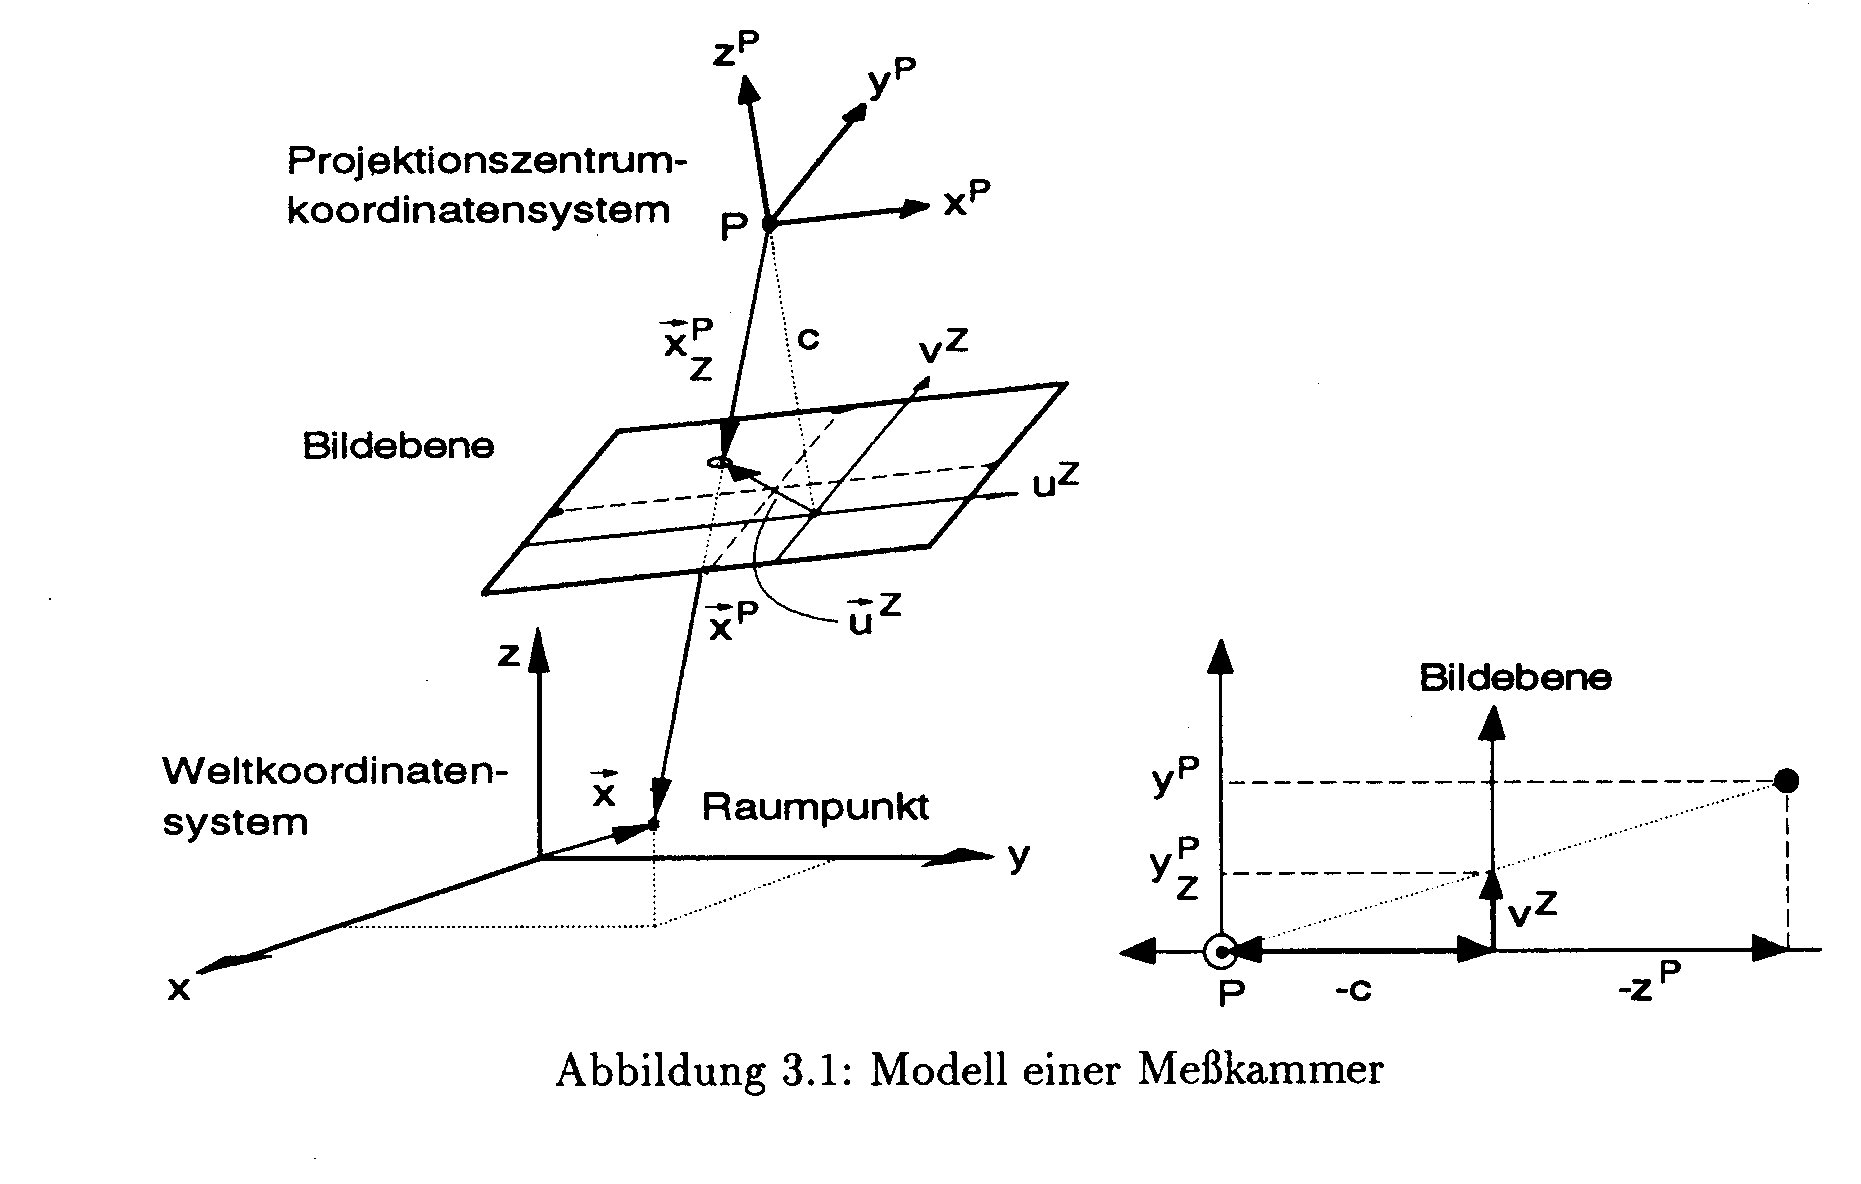
\includegraphics[width=0.65\textwidth , trim = 0mm 65mm 270mm 0mm, clip]{Bilder/cameraCalib.jpg}
			\caption{Lage des Kamerakoordinatensystems in Bezug auf Projektionsebene und Weltkoordinatensystem. \cite{Meisel:77890}}
			\label{fig:cameraCalib}
	\end{figure}

Die Kamerakalibrierung, die diesem Projekt zu Grunde liegt, ist als manuell einzustufen und kann, wenn gewünscht bzw. benötigt, zu Beginn der eigentlichen Anwendung durchgeführt werden. Um die verschiedenen Koordinatensysteme auseinander zu halten, wird zu Beginn eine Notation festgelegt, die in Tabelle~\ref{tab:camCalibParam} eingesehen werden kann. Zusätzlich können in der Tabelle sowohl die einzelnen Koordinatensysteme, als auch die einzelnen Berechnungsschritte der Kamerakalibrierung nachvollzogen werden, die im Folgenden erläutert werden. Lässt man die ersten zwei Zeilen der Tabelle weg, so ist eine Transformation von Weltkoordinaten $\vv{x}$ in Kamerakoordinaten $\vv{u}$ schematisch dargestellt. Dieses Schema muss für die Kamerakalibrierung von \textit{MaRC} invertiert werden und um die Koordinatentransformation in Unitykoordinaten ergänzt werden.  \\

\begin{table}
	\centering
	\renewcommand{\arraystretch}{1.4}
	\begin{tabular}{|c|c|c|c|}
		\hline
		\Absatzbox{}
		& \textbf{Koordinaten} & \textbf{Komponenten}&\textbf{Transformation}\\
		\hline
		$\vv{x}^U$ & Unity &$x^U$,$y^U$,$z^U$& \\
		\cline{2-4}
		$\downarrow$ & & & Koordinatentransformation\\
		\cline{2-4}
		$\vv{x}$ & Welt &$x$,$y$,$z$&  \\
		\cline{2-4}
		$\downarrow$ & & & Koordinatentransformation\\
		\cline{2-4}
		$\vv{x}^P$ & Projektionszentrum &$x^P$,$y^P$,$z^P$& \\
		\cline{2-4}
		$\downarrow$ & & & Projektion \\
		\cline{2-4}
		$\vv{x}^P_Z$ & Projektionszentrum &$u^Z$,$v^Z$,$-c$& \\
		\cline{2-4}
		$\downarrow$ & & & Linsenverzeichnung\\
		\cline{2-4}	
		$\vv{x}^P_D$ & Verzeichnung &$u^D$,$v^D$,$-c$& \\
		\cline{2-4}
		$\downarrow$ & & & Bildebenenverkippung\\
		\cline{2-4}		
		$\vv{x}^V$ &Verkippung &$u^V$,$v^V$,$-c^V$& \\
		\cline{2-4}
		$\downarrow$ & & & Bildhauptpunktverschiebung\\
		\cline{2-4}	
		$\vv{u}$ & Sensor &$u$,$v$ & \\
		\hline
	\end{tabular}
	\caption{Parameter und Berechnungsschritte der Kamera Kalibrierung.\cite{Meisel:77890}}
	\label{tab:camCalibParam}
\end{table}

Die einzelnen Schritte aus Tabelle~\ref{tab:camCalibParam} kann man in vier bzw. drei Abschnitte einteilen: \\
Im ersten Abschnitt wird der Hauptpunkt so versetzt, dass der Koordinatenursprung des Kamerakoordinatensystems mit dem Bildkoordinatensystem übereinstimmt. Dies geschieht, indem man für die eine Achse $u^V = u - \Delta u$ und für die andere Achse entsprechend $v^V = v - \Delta v$ berechnet.\\
Zusätzlich wird die Bildebene verkippt, so dass gilt $\vv{x}^V = R_v \cdot \vv{x}^P_D$. Bezeichnet $\varphi$ den Drehwinkel um die $x^P$-Achse und $\vartheta$ den Drehwinkel um die $y^{P'}$-Achse, so lässt sich $R_v$ wie folgt berechnen:

\begin{equation}
\label{equ:Rverkippt}
R_v = 
\begin{pmatrix}
r_{v11} & r_{v12} & r_{v13} \\
r_{v21} & r_{v22} & r_{v23} \\
r_{v31} & r_{v32} & r_{v33} \\
\end{pmatrix} = 
\begin{pmatrix}
\cos\vartheta & \sin\vartheta \sin\varphi & -\sin\vartheta \cos\varphi \\
0 & \cos\varphi & \sin\varphi\\
\sin\vartheta & -\cos\vartheta \sin\varphi & \cos\vartheta \cos\varphi \\
\end{pmatrix} 
~ ~ ~ ~ ~R_v \in \mathbb{R}^{3x3}
\end{equation}

Die negative verkippte Kamerakonstante $-c^V$, die in Tabelle~\ref{tab:camCalibParam} aufgeführt ist, berechnet sich wie in~\citep{Meisel:77890} beschrieben nach der Formel:

\begin{equation}
-c^V = - \frac{c+u^V \cdot r_{v13} + v^V \cdot r_{v23}}{r_{v33}}
\end{equation}

Im zweiten Schritt wird im Allgemeinem die Linsenverzeichnung herausgerechnet. Im vorliegenden Fall wurde bewusst auf diesen Schritt verzichtet und die zugehörigen Entzerrungskoeffizienten werden für alle weiteren Berechnungen auf null gesetzt. Dieses Vorgehen wurde gewählt, da einige Tests gezeigt haben, dass die berechneten Entzerrungskoeffizienten stark voneinander abgewichen sind, obwohl dies beim Benutzen der gleichen Kameraeinstellungen und dem gleichen Objektiv nicht der Fall sein dürfte.\\
Weil wie bereits beschrieben, die Linsenverzeichnung vernachlässigt wurde, kann man Schritt 1 und 2 zu einem Schritt zusammenfassen und vereinfacht darstellen. Dieser erste Schritt, also die Hauptpunktverschiebung und Bildebenenverkippung, lässt sich mit Hilfe der intrinsischen Kameramatrix $M_{intrinsisch}$ zusammenfassen. Diese beinhaltet neben den Brennweiten $f_u$ und $f_v$ noch die Koordinaten des Hauptpunktes $u^V$ und $v^V$ in Bildkoordinaten und hat somit vier Freiheitsgrade.

\begin{equation}
\label{equ:intrinsic}
M_{intrinsisch} = 
\begin{pmatrix}
f_u & 0 & 0 & u^V \\
0 & f_v & 0 & v^V\\
0 & 0 & 1 & 0 \\
\end{pmatrix} 
~ ~ ~ ~ ~M_{intrinsisch} \in \mathbb{R}^{3x4}
\end{equation}

Zu diesem Zeitpunkt sollte nun das Kamerakoordinatensystem mit dem Weltkoordinatensystem übereinstimmen und es kann sich im nächsten Schritt darum gekümmert werden, dass das Kamerakoordinatensystem verschoben und gedreht wird. Dieser Schritt und alle weiteren Schritte, die im Zusammenhang mit der Transformation von Kamerakoordinaten in Weltkoordinaten bzw. Weltkoordinaten in Unitykoordinaten stehen, werden in Kapitel~\ref{sec:planeCalib} erläutert. Hierbei sei noch einmal angemerkt, dass eine Kamerakalibrierung nur mit anschließender Kalibrierung des Arbeitsbereiches durchgeführt werden kann.


\subsubsection{Kalibrierung des Arbeitsbereichs}\label{sec:planeCalib} \todo[inline, color=yellow]{Laura}
Wie bereits beschrieben, kann eine Kalibrierung des Arbeitsbereichs entweder mit vorheriger Kamerakalibrierung oder einzeln durchgeführt werden. In letzterem Fall wird dann die zuletzt verwendete Kamerakalibrierung geladen. Die Durchführung der Kalibrierung wird in der ReadMe-Datei (vgl.~\ref{sec:readMe}) erläutert. Grob gesagt, werden über Knopfdruck am Kalibrierungscontroller (vgl. \ref{fig:KontrollerMarc}) 25 seiner Positionen sowohl in Kamerakoordinaten, als auch in Unitykoordinaten gespeichert. Man erhält also 25 korrespondierende Punktepaare.\\
Allgemein betrachtet hat die Arbeitsbereichskalibrierung zwei verschiedene Aufgaben: Zum Einen wird hierbei ein Bereich festgelegt, indem die Objekte getracked werden und zum anderen wird mittels der verschiedenen Positionen der Kalibrierungspunkte, die affine Transformationsmatrix bestimmt, die im weiteren Verlauf als Umrechnung zwischen Kamerakoordinaten und Unitykoordinaten fungiert. Beide Teilbereiche werden in den Absätzen \grqq Begrenzung des Abeitsbereichs\grqq ~bzw. \grqq Affine Transformation\grqq ~weitergehend erläutert.
	
\begin{description}
\item[Begrenzung des Arbeitsbereichs] %4 PunktepaareThe user have to make sure to form up a rectangle which is equal to his desired workspace. Starting in the lower left corner and going clockwiseÜber die ersten ... rausziehen setzt auf Null; 
\item[Affine Transformation] %21 Punktepaare.
\end{description}


\textcolor{red}{Muss noch umgeschrieben werden: }
Während eine dreidimensionale Rotation im Allgemeinen mit Matrix $R$ aus Formel~\ref{equ:Rotation} beschrieben werden kann, reicht für die Translation ein Vektor, wie $t$ aus Formel~\ref{equ:Translation} aus.\

\begin{equation}
\label{equ:Rotation}
R= R_\gamma ~R_\beta ~R_\alpha =
\begin{pmatrix}
r_{11} & r_{12} & r_{13} \\
r_{21} & r_{22} & r_{23} \\
r_{31} & r_{32} & r_{33} \\
\end{pmatrix}
~ ~ ~ ~ ~R \in \mathbb{R}^{3x3}
\end{equation}



\begin{equation}
\label{equ:Translation}
t=
\begin{pmatrix}
t_x & t_y & t_z
\end{pmatrix}^T
~ ~ ~ ~ ~t \in \mathbb{R}^{3x1} 
\end{equation}

Diese beiden Transformationen können wie in Formel~\ref{equ:extrinsic} zur extrinsischen Kameramatrix $M_{etrinsisch}$ zusammengefasst werden. Diese hat sechs Freiheitsgrade, nämlich drei für den Translationsvektor $t$ und drei für die Eulerwinkel der Rotationsmatrix $R$ für die dementsprechend gelten muss $R \in SO(3)$.

\begin{equation}
\label{equ:extrinsic}
M_{extrinsisch}= 
\begin{pmatrix}
R &|& t \\
\end{pmatrix} 
~ ~ ~ ~ ~M_{extrinsisch} \in \mathbb{R}^{3x4}
\end{equation}

Schritt 1 und 2 lassen sich vereinfachen, indem man die intrinsische Kameramatrix $M_{intrinsisch}$ und die extrinsische Kameramatrix $M_{extrinisch}$ nach der Formel~\ref{equ:inAndEx} zu einer Matrix $M$ zusammenfasst.

\begin{equation}
\label{equ:inAndEx}
M = M_{intrinsisch} \cdot M_{extrinsisch}~ ~ ~ ~ ~M\in \mathbb{R}^{3x4}
\end{equation}

Die Umrechnung von Kamerakoordinaten in Weltkoordinaten kann dann mit der invertierten Matrix $M$, wie in Formel~\ref{equ:SensInWorld} berechnet werden. \

\begin{equation}
\label{equ:SensInWorld}
\vv{x} = M^{-1} \cdot \vv{u}
\end{equation}

An diesem Punkt hat man die Kamerakoordinaten vollständig in Weltkoordinaten überführt und sucht nun eine Transformationsmatrix um diese Punkte auf ihre korrespondierenden Punkte in Unitykoordinaten abzubilden. Die dazu benötigte affine 3D-Transformation wird in Kapitel \ref{sec:planeCalib} erläutert.


%Entsprechend Formel~\ref{equ:SensInWorld} muss für den letzten Schritt eine Transformationsmatrix von Weltkoordinaten in Unitykoordinaten gefunden werden. Dies geschieht indem man die korrespondierenden Koordinatenpaare einer Controllerposition in Unity und in bereits in Weltkoordinaten gebrachten Sensorkoordinaten ineinander überführt, d.h. eine affine Transformation durchführt. Die Controlerpositionen in Weltkoordinaten werden somit auf die in Unitykoordinaten abgebildet.
\subsubsection{Kalibrierungsfehler} \label{sec:calibError}\todo[inline, color=yellow]{Laura}
In den Kapiteln~\ref{sec:camCalib} und~\ref{sec:planeCalib} wird der Algorithmus zur Berechnung der Koordinatentransformation von Kamerakoordinaten in Unitykoordinaten beschrieben. Beim Benutzen des fertig kalibrierten System fällt jedoch auf, dass die Aluminiumwürfel nicht an allen Positionen auf dem Spielfeld deckungsgleich mit ihrem gerenderten Pendant sind.  Bei genauerer Betrachtung \textcolor{red}{...Wie sieht Fehler aus? immer noch an kalibrierten Ecken und Diagonale ok?}\\
Im nächsten Kapitel werden mögliche Gründe für diese fehlerhafte Abbildung aufgeführt und diskutiert. 


\subsubsection{Mögliche Fehlerquellen} \label{sec:calibErrorSources}\todo[inline, color=yellow]{Laura}
Bei der Registrierung der Würfelobjekte kommt es zu dem in~\ref{sec:calibError} beschriebenen Fehler.
Neben der Rechenungenauigkeit und Rundungsfehlern, die sich über die diversen Rechenschritte (siehe Kapitel \ref{sec:camCalib} und \ref{sec:planeCalib}) hinweg aufaddieren, sollen in diesem Kapitel systembedingte mögliche Fehlerquellen aufgeführt werden. \\


1) Zum Einen Tracking Vive
2) Lösen DLT
3) Fehlerfortpflanzung
4) Inside out
5) Trackingfehler
6) Kamerauflösung begrenzt


Zusätzliche Registrierungsfehler können durch Latenz entstehen. Nämlich immer dann, wenn eine Zeitdifferenz zwischen der Messung der Position in Kamerakoordinaten und der eigentlichen Darstellung nach entsprechender
Verarbeitung entsteht. Solche Systemverzögerungen werden allerdings nur bei Bewegungen sichtbar und sind deshalb für die beobachteten Fehler bei ruhendem Aluminiumwürfel nicht als mögliche Fehlerquelle auszumachen.  
\subsection{Marker Detektion}
\subsection{Green Keying}\todo[inline]{Vera}
\subsection{ArUco Marker Tracking}\todo[inline]{Vera}

\subsection{Marker Objekt}\todo[inline]{Vera}
\subsection{Zuordnung der Identitäten}\todo[inline]{Vera}

\newpage